\documentclass{unina_doc_class}
\pgfplotsset{compat=1.18}
\gdef\documentname{Algebra}
\gdef\documentyear{A.A\ 2023-2024}
\gdef\xauthors{\href{giorgio99difusco@gmail.com}{\hi{\iuser Giorgio Di Fusco}}}
\gdef\yauthors{Mario Majorano, Andrea Di Donato, Luigi Ruggiero, Luigi Ferrara, Mattia Perna}
\pagestyle{plain}
\begin{document}
 \coverpage{26}{\documentyear}{30}{\documentname}
  % Chapter 0: Introduction
  \chapter{Introduzione}
\introduction{G. Cutolo}{}

\newpage

\section{Sulle versioni del documento}

\warning{Attento}{
	\textbf{Esistono diverse versioni di questo documento in circolazione}. È fondamentale assicurarsi di \textbf{consultare sempre la versione più recente}, in quanto potrebbe contenere informazioni aggiornate o correzioni rispetto alle versioni precedenti. Per evitare di studiare da fonti non esatte si raccomanda vivamente di verificare la data di pubblicazione e il numero di revisione riportati alla fine di questa pagina.
}

\begin{minipage}{.45\textwidth}
	\begin{center}
		\begin{tblr}{
			colspec = {c|c},
			hlines,
			vlines,
			row{1} = {font=\bfseries, primary!80},
			width = \linewidth
		}
		Revisione & Data \\
		\SetRow{red9} 67dfc7c & 15/03/2024 \\
		\SetRow{red9} 00a8221 & 28/08/2024 \\
		\SetRow{red9} 343cc71 & 29/08/2024  \\
		\SetRow{red9}9087dcf & 11/09/2024  \\
		\SetRow{yellow9} 83a3f0f & 01/10/2024 \\
		\SetRow{yellow9} 3af1354 & 19/02/2025 \\
		\SetRow{yellow9}  3d59ec1 & 05/09/2025 \\
		\SetRow{green9}  6a13asd & 04/10/2025
	\end{tblr}
	\captionof{table}{Cronologia revisioni del documento}
	\end{center}
\end{minipage}
\hfil
\begin{minipage}{.45\textwidth}
	\begin{center}
		\includegraphics[scale=.35]{sources/Semaforo.drawio}
	\end{center}
\end{minipage}


\section{Repository del progetto}
Tutte le versioni del documento, insieme al codice sorgente e ai materiali aggiuntivi, sono disponibili nella \href{https://github.com/Giordi9902/unina_algebra_notes}{repository} ufficiale su GitHub.

Ti invitiamo a consultare la repository per eventuali aggiornamenti, contributi o per segnalare problemi direttamente tramite issue.

\subsection{In caso di errori}
È sempre ben gradito ricevere feedback.

\textbf{Feedback generali:} se hai domande rispetto qualsiasi aspetto del libro non esitare a contattarci:
\begin{itemize}
	\item Email: \texttt{giorgio99difusco@gmail.com} (Creatore delle dispense)
	\item Telegram: \texttt{@Iracondia} (Manutentore)
\end{itemize}

  % Chapter 1: Logica
  \tableofcontents
  \chapter{Logica rudimentale}

\section{Proposizioni logiche}
Ogni teoria matematica è espressa in un \textbf{linguaggio}, che è costituito da:
\begin{enumerate}
	\item Da un \textbf{alfabeto di simboli} che possono essere messi insieme per costruire parole (stringhe di caratteri);
	\item Da \textbf{regole sintattiche} che permettono di distinguere tra stringhe ``composte correttamente'', chiamate \textbf{formule}, e stringhe che non sono correttamente composte.
\end{enumerate}

\begin{example}
	Ad esempio, la stringa ``$0<1$'' rappresenta una formula mentre la stringa $``0<$'' no.
\end{example}
Tra le formule matematiche facciamo un'ulteriore distinzione: 

\dfn{Formula chiusa}{
	Le formule alle quali è possibile attribuire univocamente un valore di verità, \textit{vero} o \textit{falso}, vengono chiamate \textbf{proposizioni} o \textbf{formule chiuse}\index{Formula chiusa}.
}

\begin{example}
	La formula ``$x>1$'' non è una proposizione in quanto non possiamo associare un valore vero o falso in quanto \textit{dipendente} dal valore della variabile $x$.
\end{example}
\subsection{I connettivi logici}
Ogni linguaggio contiene dei simboli, mediante i quali è possibile costruire periodi più complessi a partire da blocchi atomici. Anche nella logica matematica esistono dei simboli, chiamati \textbf{connettivi logici}\index{Connettivi}, che permettono di costruire proposizioni più complesse a partire da proposizioni più semplici. I connettivi logici più comuni sono:
\begin{itemize}
	\item \textbf{Negazione}: $\neg$;
	\item \textbf{Congiunzione}: $\land$;
	\item \textbf{Disgiunzione}: $\lor$;
	\item \textbf{Disgiunzione esclusiva}: $\xor$;
	\item \textbf{Equivalenza}: $\iff$;
	\item \textbf{Implicazione}: $\implies$.
\end{itemize}
\subsubsection{Negazione}\index{Connettivi!Negazione}
La negazione di una proposizione $p$ è una proposizione che è vera quando $p$ è falsa e viceversa. La negazione di una proposizione $p$ viene indicata con $\neg p$. Il connettivo di negazione è \textbf{unario}, ovvero è un connettivo che agisce su una sola proposizione. Spesso, per visualizzare i valori di verità di una proposizione, si utilizza una tabella chiamata \textbf{tabella di verità}. 

La tabella di verità della negazione è la seguente:

\begin{center}
	\begin{tblr}{
			hlines = {0.9pt}, vlines = {0.9pt}, colspec = {X[c]X[c]X[c]},
			row{1} = {primary!80!white}}
		$p$ & $\neg p$ \\
		V & F \\
		F & V
	\end{tblr}
	\captionof{table}{Tavola di verità della negazione}\label{tab:negation}
\end{center}

\subsubsection{Congiunzione}\index{Connettivi!Congiunzione}
La congiunzione di due proposizioni $p$ e $q$ è una proposizione che è vera quando $p$ e $q$ sono vere e falsa in tutti gli altri casi. La congiunzione di due proposizioni $p$ e $q$ viene indicata con $p \land q$. Il connettivo di congiunzione è \textbf{binario}, ovvero è un connettivo che agisce su due proposizioni. La tabella di verità della congiunzione è la seguente:

\begin{center}
	\begin{tblr}{
			hlines = {0.9pt}, vlines = {0.9pt}, colspec = {X[c]X[c]X[c]},
			row{1} = {primary!80!white}}
		$p$ & $q$ & $p \land q$ \\
		V & V & V \\
		V & F & F \\
		F & V & F \\
		F & F & F
	\end{tblr}
	\captionof{table}{Tavola di verità della congiunzione}\label{tab:congiunzione}
\end{center}

\subsubsection{Disgiunzione}\index{Connettivi!Disgiunzione}
La disgiunzione di due proposizioni $p$ e $q$ è una proposizione che è vera quando $p$ o $q$ sono vere e falsa in tutti gli altri casi. La disgiunzione di due proposizioni $p$ e $q$ viene indicata con $p \lor q$. La tabella di verità della disgiunzione è la seguente:

\begin{center}
	\begin{tblr}{
			hlines = {0.9pt}, vlines = {0.9pt}, colspec = {X[c]X[c]X[c]},
			row{1} = {primary!80!white}}
		$p$ & $q$ & $p \lor q$ \\
		V & V & V \\
		V & F & V \\
		F & V & V \\
		F & F & F
	\end{tblr}
	\captionof{table}{Tavola di verità della disgiunzione}\label{tab:disgiunzione}
\end{center}

\subsubsection{Disgiunzione esclusiva}\index{Connettivi!Disgiunzione esclusiva}
La disgiunzione esclusiva di due proposizioni $p$ e $q$ è una proposizione che è vera quando $p$ o $q$ sono vere, ma non entrambe, e falsa in tutti gli altri casi. La disgiunzione esclusiva di due proposizioni $p$ e $q$ viene indicata con $p \xor q$. La tabella di verità della disgiunzione esclusiva è la seguente:

\begin{center}
	\begin{tblr}{
			hlines = {0.9pt}, vlines = {0.9pt}, colspec = {X[c]X[c]X[c]},
			row{1} = {primary!80!white}}
		$p$ & $q$ & $p \xor q$ \\
		V & V & F \\
		V & F & V \\
		F & V & V \\
		F & F & F
	\end{tblr}
	\captionof{table}{Tavola di verità della disgiunzione esclusiva}\label{tab:xor}
\end{center}

\subsubsection{Equivalenza}\index{Connettivi!Equivalenza}
L'equivalenza di due proposizioni $p$ e $q$ è una proposizione che è vera quando $p$ e $q$ hanno lo stesso valore di verità e falsa in tutti gli altri casi. L'equivalenza di due proposizioni $p$ e $q$ viene indicata con $p \iff q$. La tabella di verità dell'equivalenza è la seguente:

\begin{center}
	\begin{tblr}{
			hlines = {0.9pt}, vlines = {0.9pt}, colspec = {X[c]X[c]X[c]},
			row{1} = {primary!80!white}}
		$p$ & $q$ & $p \iff q$ \\
		V & V & V \\
		V & F & F \\
		F & V & F \\
		F & F & V \\
	\end{tblr}
	\captionof{table}{Tavola di verità dell'equivalenza logica}\label{tab:equivalence}
\end{center}

\begin{defbox}{Proposizione logica}\index{Proposizione}
	Una \textbf{proposizione logica} o \textbf{forma proposizionale} è una formula ottenuta dalla composizione di una o più formule mediante connettivi logici.
\end{defbox}

Per calcolare il valore di verità di una forma proposizionale possiamo avvalerci delle tabelle di verità oppure, come si vedrà più in avanti, usare alcune proprietà che permettono di arrivare al risultato in maniera più veloce. Infatti, data una forma proposizionale di $k$ variabili è necessario costruire una tabella di $2^{k}$ righe.

\begin{example}
	\begin{enumerate}
	\item Si voglia calcolare il valore di verità della forma $p \land (q \lor p)$, dove $p$ e $q$ sono proposizioni. La tabella di verità conterrà $2^{2}=4$ righe e sarà la seguente:
	\begin{center}
		\begin{tblr}{
				hlines = {0.9pt}, vlines = {0.9pt}, colspec = {X[c]X[c]X[c]X[c]}, cells={mode=math},
				row{1} = {primary!80!white}}
			p & q & q \lor p & p \land (q \lor p)\\
			V & V & V & V \\
			V & F & V & V \\
			F & V & V & F \\
			F & F & F & F
		\end{tblr}
	\end{center}
	
	Come si può notare, per calcolare il valore di verità della formula finale ci siamo avvalsi di una colonna intermedia.


	\item Si calcoli il valore di verità della forma $P \land (Q \lor R)$, dove $P$, $Q$ e $R$ sono proposizioni. Essendo tre le variabili proposizionali la tabella di verità avrà $2^{3}=8$ righe.
	\begin{center}
		\begin{tblr}{
				hlines = {0.9pt}, vlines = {0.9pt}, colspec = {X[c]X[c]X[c]X[c]X[c]}, cells={mode=math},
				row{1} = {primary!80!white}}
			p & q & r & q \lor r & p \land (q \lor r)\\
			V & V & V & V & V \\
			V & F & V & V & V \\
			F & V & V & V & F \\
			F & F & V & V & F \\
			V & V & F & V & V \\
			V & F & F & F & F \\
			F & V & F & V & F \\
			F & F & F & F & F
		\end{tblr}
	\end{center}

	\item Un altro esempio banale di proposizioni logicamente equivalenti è dato dalla formula $P \land P$ e $P$. Si vede infatti immediatamente dalla tabella di verità:
	
	\begin{center}
		\begin{tblr}{
				hlines = {0.9pt}, vlines = {0.9pt}, colspec = {X[c]X[c]X[c]},
				row{1} = {primary!80!white}}
			$P$ & $P \land P$ & $P \iff P \land P$\\
			V  & V & V \\
			F  & F & V
		\end{tblr}
	\end{center}
	Osservando la tavola di verità notiamo che la prima e l'ultima colonna sono uguali. Questo è dovuto al fatto che la congiunzione è un connettivo \textbf{idempotente}, ovvero che restituisce sempre il primo valore di verità quando le due proposizioni sono uguali. 
\end{enumerate}
\end{example}

\begin{defbox}{Tautologia}\index{Tautologia}
	Una forma proposizionale $\varphi$ che assume valore di verità vero in modo del tutto indipendente dai valori attribuiti alle variabili che appaiono in $\varphi$ viene chiamata \textbf{tautologia}. Dualmente, esistono forme proposizionali $\varphi$ per le quali, calcolato il valore di verità, si ottiene sempre il valore F. Queste si chiamano \textbf{contraddizioni}.
\end{defbox}

Ovviamente $\varphi$ è una contraddizione se e solo se $\neg \varphi$ è una tautologia. Una forma proposizionale che non sia né una tautologia né una contraddizione si dice \textbf{contingente}. Le tautologie sono molto utili nelle dimostrazioni. Infatti, nota la tabella di verità di una determinata formula siamo in grado di sapere la tabella di verità di una formula logicamente equivalente alla prima.

\begin{example}
\begin{enumerate}
	\item La \textbf{doppia negazione} è una tautologia. Infatti, la tabella di verità è la seguente:
	
	\begin{center}
		\begin{tblr}{
				hlines = {0.9pt}, vlines = {0.9pt}, colspec = {X[c]X[c]X[c]},
				row{1} = {primary!80!white}}
			$p$ & $\neg p$ & $\neg (\neg p)$\\
			V & F & V \\
			F & V & F
		\end{tblr}
	\end{center}
	
	La doppia negazione è molto utile per semplificare le formule proposizionali. Infatti, è possibile semplificare la formula $P \land \neg (\neg P)$ in $P \land P$ e quindi in $P$.

	\item Il \textbf{principio di non contraddizione} afferma che una proposizione non può essere vera e falsa allo stesso tempo. Questo principio può essere espresso in logica proposizionale come $\neg (p \land \neg p)$, ovvero la negazione della congiunzione di una proposizione e della sua negazione. La tabella di verità è la seguente:
	
	\medskip
	
	\begin{center}
		\begin{tblr}{
				hlines = {0.8pt}, vlines = {0.9pt}, colspec = {X[c]X[c]X[c]X[c]},
				row{1} = {primary!80!white}}
			$p$ & $\neg p$ & $p \land \neg p$ & $\neg (p \land \neg p)$\\
			V & F & F & V \\
			F & V & F & V \\
		\end{tblr}
	\end{center}
	\medskip
	
	Come si può notare, la formula è una tautologia. Analogamente, è possibile ottenere una tautologia simile utilizzando il connettivo di disgiunzione: $p \lor (\neg p)$. Esempi di questa proposizione nel parlato quotidiano possono essere: ``In questo momento piove oppure in questo momento non piove'', ``Studio l'algebra oppure non studio l'algebra'', ecc. Verità oggettive sotto qualsiasi punto di vista.
\end{enumerate}
\end{example}

\begin{propbox}
	Siano $P$ e $Q$ due forme proposizionali. $P$ e $Q$ sono logicamente equivalenti se e solo se $ (P \iff Q)$ è una tautologia.
\end{propbox}

\begin{proof}
	Banale. Siano $P$ e $Q$ due proposizioni logicamente equivalenti, si ha allora:
	\begin{center}
		\begin{tblr}{hlines,vlines,row{1}={primary!80!white},colspec={X[c]X[c]X[c]},cells={mode=math}}
			P & Q & P \iff Q \\
			V & V & V \\
			F & F & V
		\end{tblr}
	\end{center}
	e  $P \iff Q$ risulta essere quindi una tautologia. Viceversa, sia $P \iff Q$ una tautologia. Allora, per definizione di equivalenza logica, $P$ e $Q$ hanno gli stessi valori logici e quindi sono logicamente equivalenti.
\end{proof}

\subsection{Il connettivo condizionale}\index{Connettivi!Implicazione}
Il connettivo condizionale è un connettivo binario che associa due proposizioni $p$ e $q$ e restituisce una proposizione che è falsa quando $p$, detta ``antecedente'', è vera e $q$, detta ``conseguente'', è falsa, e vera in tutti gli altri casi. Il connettivo condizionale di due proposizioni $p$ e $q$ viene indicato con $p \implies q$. Il connettivo condizionale è anche detto \textbf{implicazione}. La tabella di verità del connettivo condizionale è mostrata nella Tabella \ref{tab:condizionale}.

\begin{center}
	\begin{tblr}{
			hlines = {0.9pt}, vlines = {0.9pt}, colspec = {X[c]X[c]X[c]},
			row{1} = {primary!80!white}}
		$p$ & $q$ & $p \implies q$ \\
		V & V & V \\
		V & F & F \\
		F & V & V \\
		F & F & V
	\end{tblr}
	\captionof{table}{Tavola di verità del connettivo condizionale.}\label{tab:condizionale}
\end{center}

\begin{example}
	Nella logica proposizionale, frasi come ``Se piove allora il Vesuvio è alto più di mille metri sul livello del mare'' hanno assolutamente senso in quanto sono delle vere e proprie formule proposizionali. Infatti, se indichiamo con $P$ la proposizione ``piove'' e con $Q$ la proposizione ``il Vesuvio è alto più di mille metri sul livello del mare'', la frase precedente può essere riscritta come $P \implies Q$.
\end{example}

\begin{osservation}
	Perché le implicazioni con antecedente falso devono essere vere? Consideriamo la frase: ``Per ogni numero intero $x$ compreso tra 1 e 3 si ha che se $x>2$ allora $x>1$''. Tutti concordiamo sul fatto che questa frase sia vera. Analizziamola: essa significa che tutte le implicazioni del tipo $x>2 \implies x>1$ ottenute sostituendo ad $x$ uno dei numeri 1, 2, 3 sono vere. Sono vere quindi le proposizioni:
	\begin{enumerate}[itemjoin={,\quad}]
		\item $\Phi_{1}$: ``$1>2 \implies 1>1$''
		\item $\Phi_{2}$: ``$2>2 \implies 2>1$''
		\item $\Phi_{3}$: ``$3>2 \implies 3>1$''
	\end{enumerate}
	In particolare risulta vera anche la proposizione $\Phi_{1}$, che è del tipo $F \implies V$. Questo è in accordo con la tabella di verità del connettivo condizionale (Tabella \ref{tab:condizionale}). Dunque le implicazioni con antecedente falso sono vere. Si osserva che sono vere anche le implicazioni con conseguente vero. In effetti, si può dire, sinteticamente, che una \textit{implicazione è vera precisamente quando il suo antecedente è falso o il suo conseguente è vero}.
\end{osservation}

\section{Proprietà dei connettivi logici}\label{proprietà_connettivi}
Esprimere una proprietà per un connettivo logico significa affermare che la tabella di verità di una formula è sempre uguale a quella di un'altra formula. In altre parole, significa affermare che le due formule sono logicamente equivalenti e quindi che la formula che esprime la proprietà è una tautologia.

\begin{propbox}
	I connettivi logici godono delle seguenti proprietà, valgono cioè le seguenti tautologie:
	\begin{enumerate}
		\item \textbf{Idempotenza:}
		\begin{eqnarray}
			p \land p &\iff& p \\
			p \lor p &\iff& p
		\end{eqnarray}
		\item \textbf{Commutatività:}
		\begin{eqnarray}
			p \land q &\iff& q \land p \\
			p \lor q &\iff& q \lor p \\
			p \xor q &\iff& q \xor p \\
			\bigl(p \iff q\bigr) &\iff& \bigl(q \iff p\bigr)
		\end{eqnarray}
		\item \textbf{Associatività}
		\begin{eqnarray}
			\bigl(p \land q\bigr) \land r &\iff& p \land \bigl(q \land r\bigr)\\
			\bigl(p \lor q\bigr) \lor r &\iff& p \lor \bigl(q \lor r\bigr)\\
			\bigl((p \iff q) \iff r\bigr) &\iff& \bigl(p \iff (q \iff r)\bigr) \label{eq:associativity_logical_equivalence}
		\end{eqnarray}
		\item \textbf{Distributività:}
		\begin{eqnarray}
			\bigl(p \land (q \lor r)\bigr) \iff \bigl((p \land q) \lor (p \land r)\bigr)\\
			\bigl(p \lor (q \land r)\bigr) \iff \bigl((p \lor q) \land (p \lor r)\bigr)
		\end{eqnarray}
	\end{enumerate}
\end{propbox}

\begin{proof}
	Per esercizio mostriamo la dimostrazione della proprietà associativa dell'equivalenza logica (\ref{eq:associativity_logical_equivalence}). La dimostrazione delle altre proprietà è lasciata al lettore. La verifica del fatto che la proprietà in questione si tratti di una tautologia è immediata se si osserva la tabella di verità \ref{tab:associativity_equivalence}.
	
	\begin{center}
		\begin{tblr}{
				hlines = {0.9pt}, vlines = {0.9pt}, colspec = {X[c]X[c]X[c]X[c]X[2,c]X[2,c]},
				row{1} = {primary!80!white}}
			$p$ & $q$ & $r$ & $p \iff q$ & $(p \iff q) \iff r$ & $p \iff (q \iff r)$ \\
			V & V & V & V & V & V \\
			V & V & F & V & V & V \\
			V & F & V & F & F & F \\
			V & F & F & F & F & F \\
			F & V & V & F & F & F \\
			F & V & F & F & F & F \\
			F & F & V & V & V & V \\
			F & F & F & V & V & V
		\end{tblr}
		\captionof{table}{}\label{tab:associativity_equivalence}
	\end{center}
	
	Si noti che $((p \iff q)\iff r)$ risulta vera se e solo se esattamente uno o tutti e tre tra $p$, $q$ ed $r$ risulta vera. 
\end{proof} 

\begin{osservation}
	Sull'associatività di $\land$ e $\lor$, si osserva che $(p\land q)\land r$ risulta vera se e solo se sono contemporaneamente vere sia $p$ che $q$ che $r$ (lo stesso vale per $r \land (q \land r)$), mentre $(p \lor q)\lor r$ è vera se e solo se è vera almeno una tra $p$, $q$ ed $r$.
	\smallskip
	
	Più in generale è possibile provare che, qualunque sia l'intero positivo $k$ le forme proposizionale in cui appaiano tutte e sole le variabili $p_{1}, p_{2}, ..., p_{k}$, delle parentesi e, tra i connettivi solo $\land$ (analogamente $\lor$) sono equivalenti tra loro. Per queste forme si può allora rinunciare all'uso delle parentesi e scrivere semplicemente: $$p_{1} \land p_{2} \land p_{3} \land ... \land p_{k}$$ oppure $$\bigwedge_{i=1}^{k}p_{i}$$ per indicare una qualunque di queste forme.
\end{osservation}

\subsection{Le leggi di De Morgan}\index{De Morgan}
Quando è che una proposizione della forma $p \land q$ è falsa? Quando (e solo quando) è falsa almeno una tra $p$ e $q$. Questo è evidente dalla tavola di verità che descrive la congiunzione. Dualmente una proposizione della forma $p \lor q$ è falsa precisamente quando sia $p$ che $q$ sono false. Tutto questo è espresso da due tautologie molto importanti, note come \textbf{leggi di De Morgan}.

\begin{propbox}[Leggi di De Morgan]	Siano $p, \ q$ due formule, valgono allora le seguenti tautologie:
	\begin{eqnarray}
		\neg (p \land q) &\iff& (\neg p) \lor ( \neg q) \\
		\neg (p \lor q) &\iff& (\neg p) \land (\neg q)
	\end{eqnarray}
\end{propbox}

\begin{proof}
	Poniamo $\alpha \coloneqq (\neg p) \land (\neg q)$, $\beta \coloneqq (\neg p) \lor (\neg q)$. Abbiamo allora:
	\begin{center}
		\begin{tblr}
			{
				hlines = {0.9pt},
				vlines = {0.9pt},
				cells={mode=math},
				row{1}={primary!80!white},
				colspec={X[c]X[c]X[c]X[c]X[c]X[c]X[c]X[c]}
			}
			p & q & p \land q & p \lor q & \neg(p \land q) &\neg(p \lor q)& \alpha & \beta \\
			V & V & V & V & F & F & F & F\\
			V & F & F & V & V & F & F & V\\
			F & V & F & V & V & F & F & V\\
			F & F & F & F & V & V & V & V
		\end{tblr}
	\end{center}
	Dunque, per negare una disgiunzione si negano i due termini che stiamo disgiungendo e, contemporaneamente, si scambiano tra loro i simboli $\lor$ e $\land$. La negazione di una congiunzione è duale. 
\end{proof}

\subsection{Le tautologie dell'implicazione}

\begin{propbox}[Tautologia della doppia implicazione]\label{prop:doppia_implicazione}
	La congiunzione di una implicazione e della corrispondente inversa equivale alla doppia implicazione. Vale cioè la tautologia:
	\begin{equation}
		(P \iff Q) \iff \bigl((P \implies Q) \land (P \impliedby Q)\bigr)
	\end{equation}
\end{propbox}

\begin{proof} È facile convincersi osservando la seguente tabella di verità:
	\begin{center}
		\begin{tblr}
			{
				hlines = {0.9pt},
				vlines = {0.9pt}, 
				colspec = {X[c]X[c]X[c]X[c]X[c]X[2,c]},
				row{1} = {primary!80!white}, 
				cells={mode=math}
			}
			p & q & p \iff q & p \implies q & p \impliedby q & (p \implies q) \land (p \impliedby q) \\
			V & V & V & V & V & V \\
			V & F & F & F & V & F \\
			F & V & F & V & F & F \\
			F & F & V & V & V & V
		\end{tblr}
	\end{center}
	che dimostra l'enunciato.
\end{proof}

\begin{osservation}\label{oss:condizionenecessariasufficiente}
	Affermare che una certa proposizione $A$ \textbf{implica} una determinata proposizione $B$ è equivalente a dire che $A$ è una \textbf{condizione sufficiente} per $B$, ovvero che la veridicità di $A$ è sufficiente per garantire la veridicità di $B$. Inoltre, affermare che $A$ implichi $B$, è equivalente a dire che $B$ è una \textbf{condizione necessaria} per $A$, ovvero che la veridicità di $B$ è necessaria per garantire la veridicità di $A$. Il connettivo $ \implies $, a differenza degli altri connettivi binari, non è commutativo. Vale a dire che le forme $P \implies Q $ e $Q \implies P$ non sono equivalenti tra di loro.
\end{osservation}

\begin{center}
	\begin{tblr}
		{
			hlines = {0.9pt},
			vlines = {0.9pt},
			colspec = {X[c]X[c]X[c]X[c]},
			row{1} = {primary!80!white},
			row{2-5}={white},
			cells={mode=math}
		}
		P & Q & P \implies Q & Q \implies P \\
		V & V & V & V \\
		V & F & F & F \\
		F & V & V & F \\
		F & F & V & V
	\end{tblr}
	\captionof{table}{Tavola di verità dell'implicazione inversa}\label{tab:impliedby}
\end{center}

Spesso si scrive ``$P \impliedby Q$'' per ``$Q \implies P$''. Si può considerare questo simbolo ``$\impliedby$'' come un ulteriore connettivo binario (\textbf{implicazione inversa}), definito appunto dall'essere $p \impliedby q$ logicamente equivalente a $q \implies p$  come mostrato nella Tabella \ref{tab:impliedby}

\begin{example}
	Consideriamo le frasi $p:$``Oggi sto sciando'' e $q:$``Oggi sono in montagna''. Date queste due proposizioni possiamo considerare l'implicazione: ``Se oggi sto sciando allora sono in montagna.'' Questa implicazione è vera, infatti lo stare in montagna è una \textbf{condizione necessaria}\index{Condizione!Necessaria} per poter sciare ma non una condizione sufficiente. Viceversa, lo stare sciando è una \textbf{condizione sufficiente}\index{Condizione!Sufficiente} per dirci che si sta in montagna. Non vale però la formula $q \implies p$. Stare in montagna, infatti, non è sufficiente per affermare che si sta sciando, potrei infatti essere in montagna per fare una passeggiata o per fare escursionismo.
\end{example}

In generale, quando valgono contemporaneamente le formule ``$(p \implies q) \land (p \impliedby q)$'' possiamo parlare di \textbf{condizioni necessarie e sufficienti}.

\begin{center}
	\begin{tblr}
		{
			hlines = {0.9pt},
			vlines = {0.9pt},
			colspec = {X[c]X[c]X[c]},
			row{1} = {primary!80!white}
		}
		$P \implies Q$ & $P \impliedby Q$ & $P \iff Q$ \\
		Se $p$ allora $q$ & Se $q$ allora $p$ & $p$ se e solo se $q$ \\
		$p$ solo se $q$ & $p$ se $q$ & $p$ è condizione necessaria e sufficiente per $q$ \\
		$p$ è condizione sufficiente per $q$ & $p$ è condizione necessaria per $q$&$q$  è condizione necessaria e sufficiente per $p$
	\end{tblr}
	\captionof{table}{Le seguenti frasi traducono la formula nell'intestazione}
\end{center}

\begin{propbox}[Implicazione come disgiunzione]
	Il connettivo condizionale può essere espresso in termini di altri connettivi. Infatti, vale la seguente tautologia:
	\begin{equation}\label{eq:implicazione_disgiunzione}
		(p \implies q) \iff \neg p \lor q
	\end{equation}
	che esprime l'implicazione mediante la disgiunzione tra la negazione dell'antecedente e il conseguente.
\end{propbox}

\begin{proof}
	La dimostrazione segue direttamente dalle tavole di verità di implicazione e disgiunzione:
	\begin{center}
		\begin{tblr}{
				hlines = {0.9pt}, vlines = {0.9pt}, colspec ={X[c]X[c]X[c]X[c]X[c]},
				row{1} = {primary!80!white},cells={mode=math}}
			p & q & (\neg p) \lor q & p \implies q \\
			V & V & V & V \\
			V & F & F & F \\
			F & V & V & V \\
			F & F & V & V
		\end{tblr}
	\end{center}
	
	Una implicazione infatti è vera se e solo se il suo antecedente è falso o il suo conseguente è vero. 
\end{proof}

Da questa tautologia se ne può facilmente dedurre un'altra, la \hypertarget{contrapposizione}{\textbf{legge di contrapposizione}}.

\begin{propbox}[Legge di contrapposizione]\index{Contrapposizione}
	Siano $p,q$ due proposizioni logiche, vale allora la seguente:
	\begin{equation}
		(p \implies q) \iff (\neg q \implies \neg p)
	\end{equation}
\end{propbox}

\begin{proof}
	Il passaggio è il seguente:
	
	\begin{align*}
		p \implies q &\iff (\neg p) \lor q & \text{\textcolor{gray}{(per la tautologia precedente)}}  \\
		&\iff q \lor (\neg p) & \text{\textcolor{gray}{(per la commutatività di $\lor$)}} \\
		&\iff \neg(\neg q) \lor (\neg p) & \text{\textcolor{gray}{(per la doppia negazione)}} \\
		&\iff \neg q \implies \neg p & \text{\textcolor{gray}{(per la tautologia precedente)}}
	\end{align*}
\end{proof}

\begin{osservation}
	La legge di contrapposizione sta alla base del ragionamento per assurdo. Se, negando la tesi, si riesce infatti a dimostrare un fatto che neghi l'ipotesi iniziale (un \textbf{assurdo}) si dimostra allora l'implicazione originale.
\end{osservation}

Altra tautologia importante è quella che mostra come negare una implicazione. Una implicazione, infatti, è falsa precisamente quando l'\textit{antecedente è vera e falso il conseguente}. Quindi vale la seguente:

\begin{propbox}[Negazione dell'implicazione]\label{prop:negazione_implicazione}
	Siano $p$ e $q$ due formule proposizionali. Vale:
	\begin{equation}\label{eq:negazione_implicazione}
		\neg (p \implies q) \iff p \land \neg q
	\end{equation}
\end{propbox}

\begin{proof}
	La dimostrazione è immediata dalla tavola di verità dell'implicazione:
	\begin{center}
		\begin{tblr}{
				hlines = {0.9pt}, vlines = {0.9pt}, colspec = {X[c]X[c]X[c]X[c]X[c]},
				row{1} = {primary!80!white},cells={mode=math}}
			p & q & p \implies q  & ( \neg(p \implies q)) & p \land (\neg q) \\
			V & V & V & F & F \\
			V & F & F & V & V \\
			F & V & V & F & F \\
			F & F & V & F & F
		\end{tblr}
	\end{center}
\end{proof}


Un'altra tautologia di uso frequentissimo è quella della \textbf{transitività dell'implicazione}. Essa afferma che se $p \implies q$ e $q \implies r$ sono entrambe vere, allora anche $p \implies r$ è vera. In altre parole, se $p$ è una condizione sufficiente per $q$ e $q$ è una condizione sufficiente per $r$, allora $p$ è una condizione sufficiente per $r$.

\begin{propbox}[Transitività dell'implicazione]
	Siano $p, \ q,\ r$ tre formule proposizionali, vale:
	\begin{equation}\label{eq:implication-transitivity}
		\bigl((p \implies q) \land (q \implies r)\bigr) \implies (p \implies r)
	\end{equation}
\end{propbox}

\begin{proof}
	La dimostrazione è immediata dalla tavola di verità dell'implicazione. 
	
	Posto $\alpha \coloneqq (p \implies q) \land (q \implies r)$ e $\beta \coloneqq \bigl((p \implies q) \land (q \implies r)\bigr) \implies (p \implies r)$, abbiamo:
	
	\begin{center}
		\begin{tblr}{
				hlines = {0.9pt},
				vlines = {0.9pt},
				colspec = {cccccX[2,c]cX[4,c]},row{1} = {primary!80!white},cells={mode=math}}
			p & q & r & p \implies q & q \implies r & \alpha & (p \implies r) &  \beta \\
			V & V & V & V & V & V & V & V\\
			V & V & F & V & F & F & F & V\\
			V & F & V & F & V & F & V & V\\
			V & F & F & F & V & F & F & V\\
			F & V & V & V & V & V & V & V\\
			F & V & F & V & F & F & V & V\\
			F & F & V & V & V & V & V & V\\
			F & F & F & V & V & V & V & V
		\end{tblr}
	\end{center}
	
	
	Un modo alternativo per dimostrare la transitività dell'implicazione è il seguente: provare che la formula~\ref{eq:implication-transitivity} non può risultare falsa in nessun caso. Perché la formula sia falsa occorre che sia vero l'antecedente $((p \implies q) \land (q \implies r))$ e falso il conseguente $(p \implies r)$. La prima condizione significa che sono vere $(p \implies q)$ e $(q \implies r)$ per via del connettivo $\land$, la seconda che sia vera $p$ e falsa $r$.
	
	Ora, assumendo queste condizioni, sono in particolare vere $p$ e $q$ (se $p$ fosse vera e $q$ falsa allora $p \implies q$ non sarebbe potuta essere vera). Quindi, se la nostra formula è falsa, risultano vere $p$ e $q$, ma falsa $r$. Tuttavia, in questo caso, $q \implies r$ è falsa, mentre si era detto che, perché la formula sia falsa, $q \implies r$ deve essere vera. Questo ragionamento porta così ad una contraddizione che mostra che la formula considerata, cioè: $$((p \implies q) \land (q \implies r)) \implies (p \implies r)$$ non può essere falsa in nessun caso, quindi la \ref{eq:implication-transitivity} è una tautologia.
\end{proof}

L'idea esemplificata da questa dimostrazione consiste in questo: imporre che una implicazione sia falsa fornisce immediatamente due informazioni: il valore di \textit{verità dell'antecedente} ed il \textit{valore di verità del conseguente}. Dunque può essere conveniente, nello studiare una implicazione, analizzare subito le conseguenze nell'ipotesi che essa sia falsa.

Dalla transitività dell'implicazione e dalla tautologia della doppia implicazione si possono dedurre molte altre tautologie che coinvolgono i connettivi $\implies$,$\impliedby$ e $\iff$, come ad esempio la \textbf{transitività dell'equivalenza}.

\begin{propbox}[Transitività dell'equivalenza]
	Siano $p,q,r$ tre proposizioni, vale allora:
	\begin{equation}
		\bigl((p \iff q) \land (q \iff r)\bigr) \implies (p \iff r)
	\end{equation}
\end{propbox}

\begin{propbox}[Negazione di $\iff$]
	Vale questa utilissima serie di tautologie, che si possono esprimere come catena di equivalenze:
	\begin{eqnarray}
		(\neg(p \iff q)) &\iff& (\neg p \iff q) \label{eq:negation-implication}\\
		&\iff& (p \iff \neg q) \label{eq:negation-implication-2}\\
		&\iff& (p \xor q) \label{eq:negation-implication-3}
	\end{eqnarray}
\end{propbox}

Le quattro forme proposizionali sono a due a due logicamente equivalenti. Ciascuna di esse è vera quando e solo quando $p$ e $q$ hanno diversi valori di verità. La dimostrazione è lasciata al lettore come esercizio.

\subsection{Tautologie dello XOR}
Grazie a questa proposizione è possibile dimostrare la \textbf{proprietà associativa della disgiunzione esclusiva} (Formula \ref{eq:associativity_xor}):

\begin{propbox}[Associatività di $\xor$]
	Siano $p,q,r$ tre proposizioni. Allora vale la seguente tautologia:
	\begin{equation}\label{eq:associativity_xor}
		\bigl((p \xor q) \xor r\bigr) \iff \bigl(p \xor (q \xor r)\bigr)
	\end{equation}
\end{propbox}

\begin{proof}
	Consideriamo la seguente catena di equivalenze:
	\begin{align*}
		p \iff ( q \iff r) &\iff  \neg\bigl(\neg(p \iff (q \iff r))\bigr) & \textcolor{gray}{\text{(per la tautologia della doppia negazione)}} \\
		&\iff  \neg\bigl(p \iff (\neg(q \iff r))\bigr) & \textcolor{gray}{\text{(per la formula~\ref{eq:negation-implication})}}\\
		&\iff \neg\bigl(p \iff (q \xor r)\bigr) & \textcolor{gray}{\text{(per la formula~\ref{eq:negation-implication-3})}}\\
		&\iff  p \xor ( q \xor r) & \textcolor{gray}{\text{(per la formula~\ref{eq:negation-implication-3})}}\\
	\end{align*}
	Allo stesso modo si verifica la tautologia:
	\begin{equation}\label{eq:xor2}
		\bigl((p \xor q)\xor r\bigr)\iff \bigl((p \iff q) \iff r\bigr)
	\end{equation}
	Da queste due, e dall'associatività di $\iff$ si ricava la tautologia che volevamo provare.
\end{proof}

Altre due facili tautologie che riguardano la disgiunzione esclusiva sono espresse nella seguente catena di implicazioni che dimostrano l'esplicitazione del connettivo $\xor$ in termini di altri connettivi:

\begin{propbox}[Esplicitazione del connettivo $\xor$]
	Valgono le seguenti equivalenze:
	\begin{eqnarray}
		(p \xor q) &\iff& \bigl(p \land \neg(q)\bigr) \lor \bigl(q \land \neg(p)\bigr) \label{eq:exclusive-or-1}\\
		&\iff& (p \lor q) \land \bigl(\neg(p) \lor \neg(q)\bigr) \label{eq:exclusive-or-2}
	\end{eqnarray}
\end{propbox}
\begin{proof}
	Queste equivalenze si provano facilmente osservando che, evidentemente, sia
	$(p \land( \neg q)) \lor (q \land (\neg p))$ che $(p \lor q) \land ( \neg(p \land q))$ sono vere se e solo se esattamente una tra le proposizioni $p$ e $q$ è vera.
\end{proof}

\begin{propbox}[Distributività di $\land$ rispetto a $\xor$]
	Siano $a,b,c$ proposizioni logiche, vale allora:
	\begin{equation}\label{eq:distributività_congiunzione_xor}
		a \land (b \xor c) \iff (a \land b) \xor (a \land c)
	\end{equation}
\end{propbox}

\begin{proof} 
	Per dimostrare la Formula \ref{eq:distributività_congiunzione_xor} senza usare tavole di verità possiamo usare le tautologie algebriche degli operatori logici visti finora. Abbiamo quindi:
	\begin{align*}
		a \land (b \xor c) &\iff a \land \bigl((b \land \neg c ) \xor (\neg b \land c)\bigr) & \text{\textcolor{gray}{Per la tautologia \ref{eq:exclusive-or-1}}} \\
		&\iff \bigl(a \land (b \land \neg c) \bigr) \lor \bigl(a \land (\neg b \land c)\bigr) & \text{\textcolor{gray}{Per la distributività di $\land$ rispetto a $\lor$}} \\
		&\iff (a \land b \land \neg c) \lor (a \land \neg b \land c) & \text{\textcolor{gray}{Semplificando}}
	\end{align*}
	Ora consideriamo l'espansione a destra della Formula \ref{eq:distributività_congiunzione_xor} che dobbiamo dimostrare essere uguale:
	\begin{align*}
		(a \land b) \xor (a \land c) &\iff \bigl((a \land b) \land \neg(a \land c)\bigr) \lor \bigl(\neg(a \land b) \land (a \land c)\bigr) \\
		&\iff \bigl((a \land b) \land (\neg a \lor \neg c)\bigr) \lor \bigl((\neg a \lor \neg b) \land (a \land c)\bigr) \\
		&\iff \bigl((a \land b \land \neg a) \lor (a \land b \land \neg c)\bigr) \lor \bigl((\land a \land a \land c) \lor (\neg b \land a \land c)\bigr) \\
		&\iff (a \land b \land \neg c) \lor (a \land \neg b \land c)
	\end{align*}
	Notiamo ora che entrambi i lati dell'equazione sono uguali e la dimostrazione può dirsi conclusa.
\end{proof}

\section{I quantificatori}\index{Quantificatore}

\subsection{Formule e quantificatori}
Consideriamo la formula ``$x>1$'' del linguaggio naturale. Questa formula, pur avendo un senso compiuto, non è una \textbf{proposizione}, ovvero non è possibile determinare per essa un valore di verità. Espressioni del genere possono essere generalizzate nel modo seguente: \[\varphi(x):\mbox{``Espressione della variabile $x$"}\]
E così via:
\begin{displaymath}
	\varphi(x_{1},...,x_{n}) : \mbox{``Espressione delle variabili $x_{1},...,x_{n}$"}
\end{displaymath}

Di conseguenza, nel caso di $\varphi(x):``x>1"$ se $x=3$ allora $\varphi(3)=``3>1"$ che è una proposizione, in particolare vera. Da questo breve esempio possiamo estendere la nozione di verità, valutando la formula per ciascuno dei valori che possono essere \emph{sostituiti} alla variabile $x$.

\begin{defbox}{Formula valida}
	Una formula che risulta vera per ogni possibile sostituzione delle variabili si dice \textbf{valida}.
\end{defbox}
La nozione di sostituzione permette di introdurre due nuovi simboli logici che svolgono un ruolo centrale nel \textbf{calcolo dei predicati}. Questi simboli sono i \textbf{quantificatori}.

\begin{defbox}{Quantificatore universale}\index{Quantificatore!Universale}
	Se $\varphi$ è una formula ed $x$ è una variabile allora anche ``$\forall x(\varphi)$'' è una formula, chiamata \textbf{formula universale} e si legge ``per ogni $x$, $\varphi$ è vera''. Questa formula esprime la contemporanea affermazione di tutte le formule $\varphi(a)$ ottenute sostituendo ad $x$ ogni possibile valore $a$.
	Il simbolo $\forall$ prende il nome di \textbf{quantificatore universale}.
\end{defbox}

\begin{osservation}
	Sono equivalenti le forme: $\forall x \ \bigl( \varphi(x) \bigr)$ e $\forall x(\varphi)$. A volte, per esplicitare la parte del quantificatore si usa racchiuderlo tra parentesi tonde: $(\forall x) (\varphi(x))$.
\end{osservation}

\begin{example}
	Sia $\varphi : x > 3$ e sia l'universo del discorso ristretto all'insieme dei numeri naturali, allora scrivere ``$\forall x \bigl(\varphi(x)\bigr)$'' equivale a dire ``per ogni numero naturale $x$, questo è maggiore di 3'' che ovviamente è falso.
\end{example}

\begin{osservation}
	Il quantificatore universale può essere visto\footnote{La congiunzione però non può operare su un numero infinito di proposizioni mentre il quantificatore si.} come una sequenza di proposizioni collegate tra di loro con un connettivo di congiunzione.
\end{osservation}

Se le formule universali possono essere pensate come una sorta di congiunzione generalizzata, le \textbf{formule esistenziali}, cioè quelle del tipo ``$\exists x(\varphi)$'' (che si legge ``esiste un $x$ tale che $\varphi$ è vera'') possono essere pensate come disgiunzioni generalizzate.

\begin{defbox}{Quantificatore esistenziale}\index{Quantificatore!Esistenziale}
	Se $x$ è una variabile e $\varphi = \varphi(x)$ una formula, $\exists x(\varphi)$ esprime l'affermazione di \textit{almeno una} tra le formule $(\varphi(a))$ ottenute sostituendo ad $x$ ogni possibile valore $a$.
	Il simbolo $\exists$ prende il nome di \textbf{quantificatore esistenziale}.
\end{defbox}

Oltre a $\forall$ e $\exists$ esistono altri quantificatori. Quello di uso più frequente è $\exists!$. Se $\varphi$ è una formula ed $x$ è una variabile, la formula ``$\exists!x(\varphi)$'' si legge ``esiste uno ed un solo $x$ tale che $\varphi$'' ed afferma $\varphi(a)$ per uno dei possibili valori $a$ che possono essere sostituiti ad $x$, negando $\varphi(b)$ per ogni $b$ diverso da a. In modo più sintetico e più formale, se $y$ è una variabile (diversa da $x$) che non appare in $\varphi$, questo quantificatore è definito dall'equivalenza:
\begin{equation}
	\exists! x(\varphi(x)) \ \iff \ \exists x(\forall y(\varphi(y)\iff y=x))
\end{equation}

Siano $\varphi$ una formula e $x,y$ due variabili, e assumiamo che $y$ non appaia in $\varphi$. Se chiamiamo $\psi(x,y)$ la formula $$\varphi(y) \iff y=x$$possiamo riscrivere l'equivalenza come:
\begin{displaymath}
	\exists! x(\varphi(x)) \ \iff \ \exists x(\forall y(\psi(x,y)))
\end{displaymath}

Vogliamo esaminare il membro a destra di questa equivalenza. Supponiamo che $\varphi$ sia un predicato unario in $x$, quindi che $\exists x (\forall y (\psi(x,y)))$ sia una proposizione. Quando è che questa proposizione è vera? Esattamente quando esiste almeno un $a$ per il quale sia vera la formula $\forall y(\phi(a,y))$; questo equivale a dire che è vera $\psi(a,b)$, cioè la formula $\varphi(b) \iff b=a$, per ogni possibile scelta di $b$.

Tra le possibili scelte per $b$ c'è anche $a$; la formula diventa in questo caso particolare $\varphi(a) \iff a = a$. Poiché $a=a$ è vera, questa equivale a $\varphi(a)$. Se invece scegliamo come $b$ un qualsiasi oggetto diverso da $a$, allora $b=a$ è falsa, quindi $\varphi(b)\iff b=a$ equivale alla negazione di $\varphi(b)$.

In definitiva, abbiamo mostrato che la formula $\exists x(\forall y(\psi(x,y)))$ è vera se e solo se esiste un $a$ per il quale è vera $\varphi(a)$ e, contemporaneamente, è falsa $\varphi(b)$ per ogni $b$ diverso da $a$. Questo è precisamente quello che si vuole esprimere con il quantificatore $\exists!$.

\subsection{Occorrenze libere e vincolate}
In una formula come:
\[
\forall x \bigl( \ldots \bigr)
\]
o come
\[
\exists x \bigl( \ldots \bigr)
\]
si dice che le \textit{occorrenze} della variabile $x$ all'interno dello \textit{scope del quantificatore} (ovvero la parte della formula logica o del programma in cui il quantificatore è efficace) sono \textbf{vincolate}\index{Occorrenza!Vincolata} dal quantificatore $\forall$ o dal quantificatore $\exists$.

\begin{defbox}{Occorrenza libera}
	Una variabile che non è vincolata da alcun quantificatore si dice ad \textbf{occorrenza libera}\index{Occorrenza!Libera}.
\end{defbox}

\begin{example}
	Nella definizione appena data di occorrenze libere e vincolate si intende il fatto che ogni quantificatore può vincolare solo le occorrenze delle variabili che lo seguono immediatamente. In $\forall x (x=y)$ il quantificatore vincola solo le occorrenze della variabile $x$ mentre le occorrenze della variabile $y$ sono libere.
\end{example}

\begin{example}
	Sono vincolate le occorrenze di $x$ in $\forall x(x+1>x) \land (\exists x(x>y))$, mentre nella stessa formula è libera l'occorrenza di $y$.
\end{example}

\begin{example}
	In una stessa formula possono esserci sia occorrenze libere che vincolate di una stessa variabile. Ad esempio in $(\forall x(x+1>x))\lor(x=0)$ l'ultima occorrenza di $x$ è libera perché fuori dallo scope di ogni quantificatore.
\end{example}

\begin{defbox}{Formula chiusa}
	Una formula si dice \textbf{chiusa}\index{Formula!chiusa} se e solo se non contiene variabili con occorrenze libere.
\end{defbox}

\begin{example}
	Formule del tipo $\exists x(x>y)$ non sono proposizioni a causa della presenza di variabili libere. Quindi non hanno un valore di verità. Per poter attribuire un valore di verità bisogna prima ``quantificare" le variabili libere che vi appaiono facendo opportune modifiche.
\end{example}

\subsection{Sostituzioni}\index{Sostituzione}
Per quanto riguarda le \textit{sostituzioni} invece va detto che queste coinvolgono solo e soltanto le \textit{occorrenze delle variabili libere presenti}.

\begin{example}
	Sia ``$\varphi(x) : x > 1$'' e consideriamo la sostituzione $\varphi(5)$ ottenuta eseguendo la sostituzione della variabile $x$ con il simbolo $5$. Si ottiene quindi la formula ``$5 > 1 $'' che ha un proprio valore di verità. Consideriamo adesso la formula ``$\psi(x) : (\forall x) (x>1)$'' dove è presente una occorrenza vincolata della variabile $x$. Provando ad eseguire la sostituzione di tutte le occorrenze della variabile $x$ con il simbolo 5 si ottiene ``$ \psi(5) : \forall 5 (5>1)$'' che è una formula priva di senso.
\end{example}

È buona norma scrivere le formule in modo che le variabili appaiano solo in forma libera o vincolata. Inoltre, cambiando il nome di una variabile vincolata, se non è presente anche in forma di occorrenza libera nella formula, allora la formula non cambia il suo valore di verità.

\subsection{Predicati}\index{Predicato}

\begin{defbox}{Predicato}
	Un \textbf{predicato unario}\index{Predicato!unario} nella variabile $x$ è una formula che \textit{non contiene} occorrenze libere di variabili diverse da $x$. Similmente, si dice che la formula $\varphi$ è un \textbf{predicato binario} quando in essa appaiono al più due variabili con occorrenze libere.
\end{defbox}

\begin{example}
	La formula $x=x$ è un predicato unario nella variabile $x$ in quanto è una formula in cui occorre una sola variabile libera che è $x$. La formula $x=y$ è un predicato binario in quanto è una formula in cui occorrono due variabili libere che sono $x$ e $y$.
\end{example}

\subsection{I quantificatori ristretti}\index{Quantificatore!Ristretto}
Nella pratica matematica si incontrano spesso espressioni del tipo:
\[
(\forall x \in \mathbb{R})(\alpha(x))
\]
oppure:
\[
(\exists x>0)(\varphi)
\]
in cui il quantificatore è accompagnato da una condizione che ``limita'' l'ambiente in cui la variabile può assumere valori. Queste formule sono abbreviazioni\footnote{Anche detto allargamento del linguaggio} di formule in cui i quantificatori sono usati nel metodo tradizionale. La prima formula può essere definita in questo modo:
\[
(\forall x \in \mathbb{R})(\alpha(x)) : \iff \forall x (x \in \mathbb{R} \implies \alpha(x))
\]
\begin{example}
	Quando ci si trova davanti a formule del tipo
	\[
	\begin{array}{lc}
		\forall x \in \varnothing \; (x = x) \\
		\forall x \in \varnothing \;(x \neq x)
	\end{array}
	\]
	si stanno abbreviando formule del tipo:
	\[
	\begin{array}{lc}
		\forall x( x \in \varnothing \implies x=x) \\
		\forall x(x \in \varnothing \implies x \neq x) \\
	\end{array}
	\]
	che risultano sempre vere in quanto implicazioni con antecedente falso.
\end{example}

Espressioni come $(\exists x \in S) (\varphi(x))$ abbreviano invece formule del tipo $\exists x (x \in S \land \varphi(x))$ e qui non dovrebbero esserci difficoltà: ``esiste $x$ in S tale che $\ldots$'' significa proprio che ``esiste $x$ tale che $x$ sia in S e $\ldots$ ''. Ovviamente, nella solita ipotesi che $\varphi$ sia un predicato unario in $x$, questa formula è sicuramente una proposizione falsa quando $S = \varnothing$.

\subsection{Regole di manipolazione dei quantificatori}
In matematica è molto comune trovare delle formule al cui interno sono presenti quantificatori annidati come segue:
\[
\begin{array}{lc}
	\forall x ( \forall y (\forall z ( \cdots ) ) ) \\
	\exists x ( \exists y (\exists z (\cdots )))\\
\end{array}
\]
In questi casi è comodo abbreviare usando una notazione compatta del tipo:
\[
\begin{array}{lc}
	\forall x,y,z ( \cdots ) \quad \mbox{ al posto di } \quad \forall x ( \forall y (\forall z ( \cdots ) ) ) \\
	\exists x,y,x (\cdots ) \quad \mbox { al posto di } \quad \exists x ( \exists y (\exists z (\cdots )))\\
\end{array}
\]
Le cose cambiano quando troviamo annidati sia il quantificatore esistenziale che quello universale. Le formule ``$\forall x (\exists y (\varphi))$" e ``$\exists y (\forall x (\varphi))$" non sono in generale equivalenti e non possono essere scambiate a proprio piacimento. La prima afferma che, scelto comunque un termine $a$, ne esiste almeno uno, $b$, dipendente, in generale, dalla scelta di $a$ per il quale si abbia $\varphi(a,b)$. La seconda afferma qualcosa di più: che si ha la stessa situazione ma, questa volta, si può scegliere $b$ indipendentemente dalla scelta di $a$: esiste un particolare $b$ per il quale sia abbia $\varphi(a,b)$ per ogni possibile scelta di $a$. Dunque vale sempre l'implicazione:
\begin{displaymath}
	\exists y \bigl( \forall x (\varphi) \bigr) \implies \forall x \bigl( \exists y (\varphi)\bigr)
\end{displaymath}
ma, in generale, non vale l'implicazione inversa.

\begin{example}
	Nel linguaggio dell'aritmetica, sia $\varphi(x,y)$ la formula $x<y$. La prima delle nostre formule diventa:
	\begin{displaymath}
		\forall x (\exists y (x<y))
	\end{displaymath}
	che afferma che per ogni numero esiste un numero più grande. Questa è una proposizione vera: se $a$ è un numero intero, $a+1$ è un numero intero maggiore di $a$, quindi $\varphi(a,a+1)$ è vera. La seconda formula è invece:
	\begin{displaymath}
		\exists y (\forall x (x < y))
	\end{displaymath}
	che afferma che esiste un intero (quello che andrebbe sostituito ad $y$) maggiore di tutti gli interi; questa è una proposizione falsa.
\end{example}

\subsection{Negazione dei quantificatori}
\begin{propbox}\label{prop:negazione_quantificatori}
	Valgono le seguenti equivalenze logiche:
	\begin{eqnarray}
		\neg(\forall x (\varphi(x))) \iff (\exists x (\neg \varphi(x))) \label{eq:negazione_universale}\\
		\neg(\exists x (\varphi(x))) \iff (\forall x (\neg \varphi(x))) \label{eq:negazione_esistenziale}
	\end{eqnarray}
\end{propbox}
\begin{proof}
	Lasciata al lettore come esercizio.
\end{proof}

Queste regole valgono in maniera analoga per i quantificatori ristretti con le dovute osservazioni:
\begin{eqnarray*}
	\neg(\forall x \in S(\varphi(x))) &\iff & \neg (\forall x (x \in S \implies \varphi(x)))  \\
	&\iff & \exists x (\neg (x \in S\implies \varphi(x))) \\
	&\iff & \exists x (x \in S \land \neg \varphi(x))
\end{eqnarray*}
Analogamente:
\begin{eqnarray*}
	\neg (\exists x \in S(\varphi(x))) &\iff & \neg(\exists x( x \in S \land \varphi(x)))  \\
	&\iff & \forall x (\neg(x\in S \land \varphi(x))) \\
	&\iff & \forall x (\neg (x \in S) \lor (\neg \varphi(x)))
\end{eqnarray*}
\begin{propbox}
	La negazione di $\exists!$ è data dalla seguente equivalenza:
	\begin{equation}
		\neg\Bigl(\exists x\bigl(\forall y (\varphi y) \iff x=y\bigr)\Bigr) \iff
		\forall x \Bigl(\exists y \bigl(\neg (\varphi(y) \iff x=y)\bigl)\Bigr)
	\end{equation}
\end{propbox}

\begin{proof}
	Banale.
\end{proof}
\newpage
\section{Esercizi svolti}
\begin{exsbox}
	Scrivere le tavole di verità di ciascuna delle forme proposizionali:
	\begin{itemize}
		\item ``$p \land p$''
		\item ``$(\neg p)\land q$''
	\end{itemize}
\end{exsbox}

\paragraph*{Svolgimento.}
\begin{center}
		\begin{tblr}{hlines = {0.9pt}, vlines = {0.9pt},row{1}={primary!80!white},colspec={X[c]X[c]X[c]},cells={mode=math}}
			p & p & p \land p \\
			V & V & V \\
			F & F & F \\
		\end{tblr}
\end{center}
\begin{center}
		\begin{tblr}{hlines = {0.9pt}, vlines = {0.9pt},row{1}={primary!80!white},colspec={X[c]X[c]X[c]X[c]},cells={mode=math}}
			p & q & \neg p & (\neg p) \land q \\
			V & V & F & F\\
			V & F & F & F\\
			F & V & V & V\\
			F & F & V & F
		\end{tblr}
\end{center}
\begin{flushright}
	\blacksquare
\end{flushright}

\begin{exsbox}
	Scrivere le tavole di verità delle forme proposizionali
	\begin{enumerate}
		\item ``$p \land(q \land r)$''
		\item ``$p \land (q \land(\neg r))$''
	\end{enumerate}
\end{exsbox}

\paragraph*{Svolgimento.}
\begin{center}
		\begin{tblr}{hlines, vlines,row{1}={primary!80!white},colspec={X[c]X[c]X[c]X[c]X[2,c]},cells={mode=math}}
			p & q & r & q \land r & p \land (q \land r) \\
			V & V & V & V & V \\
			V & V & F & F & F \\
			V & F & V & F & F \\
			V & F & F & F & F \\
			F & V & V & V & F \\
			F & V & F & F & F \\
			F & F & V & F & F \\
			F & F & F & F & F
		\end{tblr}
\end{center}

\begin{center}
\begin{tblr}{hlines = {0.9pt}, vlines = {0.9pt},row{1}={primary!80!white},colspec={X[c]X[c]X[c]X[c]X[2,c]X[3,c]},cells={mode=math}}
			p & q & r & \neg r & q \land (\neg r) & p \land \bigl(q \land (\neg r)\bigr) \\
			V & V & V & F & F & F \\
			V & V & F & V & V & V \\
			V & F & V & F & F & F \\
			V & F & F & V & F & F \\
			F & V & V & F & F & F \\
			F & V & F & V & V & F \\
			F & F & V & F & F & F \\
			F & F & F & V & F & F
		\end{tblr}
\end{center}

\begin{flushright}
	\blacksquare
\end{flushright}
\begin{exsbox}
	Scrivere le tavole di verità di ciascuna delle forme proposizionali:
	\begin{itemize}
		\item ``$p \land ( p \lor q)$''
	\end{itemize}
\end{exsbox}
\paragraph*{Svolgimento.}
\begin{center}
	\begin{tblr}{hlines = {0.9pt}, vlines = {0.9pt},row{1}={primary!80!white},colspec={X[c]X[c]X[c]X[c]},cells={mode=math}}
		p & q & p \lor q & p \land (p \lor q) \\
		V & V & V & V \\
		V & F & V & V \\
		F & V & V & F \\
		F & F & F & F
	\end{tblr}
\end{center}
\begin{flushright}
	\blacksquare
\end{flushright}
\begin{exsbox}
	Scrivere le tavole di verità di ciascuna delle forme proposizionali:
	\begin{itemize}
		\item $p \lor (p \land q)$
		\item $p \implies (\neg p)$
		\item $p \land (\neg q) \land r$
	\end{itemize}
\end{exsbox}
\paragraph{Svolgimento.} Abbiamo:
\begin{center}
	\begin{tblr}{hlines = {0.9pt}, vlines = {0.9pt},row{1}={primary!80!white},colspec={X[c]X[c]X[c]X[c]},cells={mode=math}}
		p & q & (p \land q) & p \lor (p \land q)\\
		V & V & V  & V \\
		V & F & V  & V\\
		F & V & F  & F\\
		F & F & F & F
	\end{tblr}
\end{center}
\begin{center}
	\begin{tblr}{hlines = {0.9pt}, vlines = {0.9pt},row{1}={primary!80!white},colspec={X[c]X[c]X[c]},cells={mode=math}}
		p & \neg p & (p \implies \neg p)\\
		V & F & F  \\
		F & V & V
	\end{tblr}
\end{center}
\begin{center}
	\begin{tblr}{hlines = {0.9pt}, vlines = {0.9pt},row{1}={primary!80!white},colspec={X[c]X[c]X[c]X[c]X[c]},cells={mode=math}}
		p & q & r & \neg q & p \land (\neg q) \land r \\
		V & V & V & F & F \\
		V & V & F & F & F \\
		V & F & V & V & V \\
		V & F & F & V & F \\
		F & V & V & F & F \\
		F & V & F & F & F \\
		F & F & V & V & F \\
		F & F & F & V & F
	\end{tblr}
\end{center}
\hfill \blacksquare
\begin{exsbox}
	Definiamo il connettivo \textbf{NAND} tra due proposizioni $p$ e $q$, $p \uparrow q$ come $\neg(p \land q)$. Decidere se la forma proposizionale $(p \uparrow ( q \uparrow r)) \iff ((p \uparrow q)\uparrow r)$ è una tautologia.
\end{exsbox}
\paragraph*{Svolgimento.}È possibile dimostrare che tale formula non è una tautologia costruendo le tavole di verità. Si ha:

\begin{center}
		\begin{tblr}{hlines = {0.9pt}, vlines = {0.9pt},row{1}={primary!80!white},colspec={X[c]X[c]X[c]X[c]X[2,c]},cells={mode=math}}
			p & q & r & q \uparrow r & p \uparrow (q \uparrow r) \\
			V & V & V & F & V \\
			V & V & F & V & F \\
			V & F & V & V & F \\
			V & F & F & V & F \\
			F & V & V & F & V \\
			F & V & F & V & V \\
			F & F & V & V & V \\
			F & F & F & V & V
		\end{tblr}
\end{center}
\begin{center}
		\begin{tblr}{hlines = {0.9pt}, vlines = {0.9pt},row{1}={primary!80!white},colspec={X[c]X[c]X[c]X[c]X[2,c]},cells={mode=math}}
			p & q & r & p \uparrow q & (p \uparrow q) \uparrow r \\
			V & V & V & F & V \\
			V & V & F & F & V \\
			V & F & V & V & F \\
			V & F & F & V & V \\
			F & V & V & V & F \\
			F & V & F & V & V \\
			F & F & V & V & F \\
			F & F & F & V & V
		\end{tblr}
\end{center}
È possibile raggiungere lo stesso risultato ponendo $\alpha \coloneqq (p \uparrow ( q \uparrow r))$ e $\beta \coloneqq ((p \uparrow q)\uparrow r)$ e supporre che $\alpha$ sia falsa. Essendo $p \uparrow q \iff \neg(p \land q)$ si ha che $p \uparrow q$ è falsa se sono vere entrambe le proposizioni $p$ e $q$. Allora $\alpha$ è falsa se e solo se $p$ e $q \uparrow r$ sono entrambe vere. Se $q \uparrow r$ è vera, allora almeno una tra $q$ e $r$ è falsa. Se $q$ è falsa, allora $p \uparrow q$ è vera, dunque $\beta$ è vera. Se $r$ è falsa, allora $q \uparrow r$ è vera, dunque $\beta$ è vera. In entrambi i casi $\beta$ è vera, dunque $\alpha \iff \beta$ non è una tautologia. \hfill \blacksquare
\begin{exsbox}
	Scrivere le tavole di verità di ciascuna delle forme proposizionali: ``$p \implies (p \lor q)$'', ``$(p \land q) \implies r$'', ``$(p \land q) \iff r$''.
\end{exsbox}
\paragraph*{Svolgimento.} Possiamo costruire, per semplicità, una singola tabella per il calcolo delle tre proposizioni. Si ha quindi:
\begin{center}
	\begin{tblr}{hlines, vlines,row{1}={primary!80!white},colspec={X[c]X[c]X[c]X[c]X[c]X[2,c]X[2,c]X[2,c]},cells={mode=math}}
		p & q & r & p \land q & p \lor q & p \implies (p \lor q) & (p \land q) \implies r & (p \land q) \iff r \\
		V & V & V & V & V & V & V & V \\
		V & V & F & V & V & V & F & F \\
		V & F & V & F & V & V & V & F \\
		V & F & F & F & V & V & V & V \\
		F & V & V & F & V & V & V & F \\
		F & V & F & F & V & V & V & V \\
		F & F & V & F & F & V & V & F \\
		F & F & F & F & F & V & V & V
	\end{tblr}
\end{center}
\begin{flushright}
	\blacksquare
\end{flushright}
\begin{exsbox}
	Verificare se $(t \land (\neg v) \lor m) \iff (t \land (v \implies m))$.
\end{exsbox}
\paragraph{Svolgimento.} Dimostriamo costruendo la tavola di verità:
\begin{center}
	\begin{tblr}{hlines = {0.9pt}, vlines = {0.9pt},row{1}={primary!80!white},cells={mode=math},colspec={X[c]X[c]X[c]X[c]X[c]}}
		t & v & m & t \land (\neg v) \lor m & t \land (v \implies m) \\
		V & V & V & V & V \\
		V &V &F & F & F \\
		V & F & V & V & V \\
		V & F & F & V & V \\
		F & V & V & F & F \\
		F & V & F & F & F \\
		F & F & V & F & F \\
		F & F & F & F & F
	\end{tblr}
\end{center}
Confrontando le colonne si ha l'asserto. \hfill \blacksquare
\begin{exsbox}
	Stabilire i valori di verità delle formule e frasi (assumiamo nota la matematica elementare coinvolta): ``$(1+1=0)\land(0+0=0)$''; ``$(1+1=0) \lor (0+0=0)$''; ``$(1+1=0)\implies (0+0=0)$''; ``$\sqrt{2}$ è un numero razionale o un numero irrazionale''; ``$2^{5}=32 \implies 47-1=46$''.
\end{exsbox}
\paragraph*{Svolgimento.}
\begin{enumerate}
	\item ``$(1+1=0)\land(0+0=0)$'' risulta vera in quanto falsa l'antecedente.
	\item ``$(1+1=0) \lor (0+0=0)$'' risulta vera;
	\item ``$(1+1=0) \implies (0+0=0)$'' risulta vera;
	\item ``$\sqrt{2}$ è un numero razionale o un numero irrazionale'' è vera;
	\item  ``$2^{5}=32 \implies 47-1=46$'' è vera.
\end{enumerate}
\begin{flushright}
	\blacksquare
\end{flushright}

\begin{exsbox}
	È molto importante saper ``tradurre'' espressioni del linguaggio ordinario (della lingua italiana) in linguaggio ``semiformalizzato'', riconoscendo la presenza ed il ruolo dei connettivi proposizionali contenuti nelle frasi. Ad esempio, se indichiamo con $\alpha$ la frase ``domani pioverà'' e con $\beta$ la frase ``domani prenderò l'ombrello'', si può rendere con $\alpha \land \beta$ la frase ``domani pioverà e prenderò l'ombrello''. Fare lo stesso con le frasi:
	\begin{itemize}
		\item Il supermercato era aperto e non ci sono entrato.
		\item Il supermercato era aperto ma non ci sono entrato.
		\item Se vedo Nicola lo saluto.
		\item Se domenica non piove e vado a Roma, $2>1$, ma se Marco mangia la pizza allora certamente fioriranno le rose.
	\end{itemize}
\end{exsbox}
\paragraph*{Svolgimento.} Si ha:
\begin{itemize}
	\item Posto $\alpha$: ``Il supermercato era aperto'' e $\beta$: ``Ci sono entrato'' si ottiene: $\alpha \land \neg \beta$;
	\item Posto $\alpha$: ``Il supermercato era aperto'' e $\beta$: ``Ci sono entrato'' si ottiene: $\alpha \land \neg \beta$;
	\item Posto $\alpha$: ``Vedo Nicola'' e $\beta$: ``Lo saluto'' si ottiene: $\alpha \implies \beta$;
	\item Posto $\alpha$: ``Domenica piove'', $\beta$: ``Vado a Roma'', $\gamma$: ``$2>1$'', $\delta$: ``Marco mangia la pizza'' e $\zeta$: ``Fioriscono le rose'' si ottiene:
	$\Bigl( \bigl( \neg (\alpha) \land \beta \bigr) \implies \delta \Bigr) \land \bigl(\theta \implies \zeta \bigr)$.
\end{itemize}
\begin{flushright}
	\blacksquare
\end{flushright}

\begin{exsbox}
	Spiegare la seguente storiella: la moglie del logico chiede al marito: ``Caro, stasera usciamo o restiamo a casa?''. Il marito risponde ``Sì.''.
\end{exsbox}
\paragraph*{Svolgimento.} Il marito ha risposto ``sì'' perché la frase ``stasera usciamo o restiamo a casa'' è una proposizione composta da una singola proposizione logica, $p$, congiunta dalla disgiunzione esclusiva : $p \xor (\neg p)$ che risulta essere una tautologia. La risposta del marito non può essere quindi che affermativa. \hfill \blacksquare

\begin{exsbox}
	Verificare la tautologia $\bigl(p \implies (q \implies r)\bigr) \iff \bigl((p \implies q) \implies (p \implies r) \bigr)$ (distributività da sinistra dell'implicazione rispetto a sé stessa).
\end{exsbox}
\paragraph*{Svolgimento.} Sia $\alpha \coloneqq \bigl(p \implies (q \implies r)\bigr)$ e $\beta \coloneqq \bigl((p \implies q) \implies (p \implies r) \bigr)$. Verifichiamo che $\alpha \iff \beta$ non può essere mai falsa. Per essere falsa devono assumere valore diverso, per ogni valore di $p,q,r$, le due formule. Sia quindi $\alpha$ falsa e $\beta$ vera. Si ha quindi che sia $p$ che $q \implies r$ hanno valore falso. Quindi $q$ ha valore vero ed $r$ assume valore falso. In questa situazione si ha che $p \implies q$ è vera e $p \implies r$ è falsa. Quindi $\beta$ è falsa, trovando una contraddizione. Viceversa, sia $\alpha$ vera e $\beta$ falsa. Procedendo in maniera analoga si ottiene che $p$ e $q$ sono vere mentre $r$ è falsa. Allora, stando questi valori, $\alpha$ è falsa, contro le ipotesi iniziali e quindi $\alpha$ e $\beta$ non assumono mai valori logicamente diversi. \hfill \blacksquare

\begin{exsbox}
	Negare ciascuna delle frasi: ``Mario corre e Maria nuota'', ``La bottiglia è vuota oppure tappata''.
\end{exsbox}
\paragraph*{Svolgimento.} Poniamo $\alpha$:``Mario corre'' e $\beta:$ ``Mario nuota''. La frase ``Mario corre e Mario nuota'' corrisponde quindi a $\alpha \land \beta$. Per negare la frase si procede quindi nel seguente modo:
\begin{displaymath}
	\neg (\alpha \land \beta)  \iff \neg (\alpha) \lor \neg (\beta)
\end{displaymath}
ovvero: ``Mario non corre oppure non nuota''. Analogamente, posto $\alpha$: ``La bottiglia è vuota'' e $\beta$: ``La bottiglia è tappata'' si ha:
\begin{displaymath}
	\neg (\alpha \lor \beta) = \neg (\alpha) \land \neg (\beta)
\end{displaymath}
Ovvero: ``La bottiglia non è vuota e non è tappata''. \hfill \blacksquare
\begin{exsbox}
	Negare la frase: ``Alice ha i capelli biondi ricci''. (Si chiede che anche la negazione inizi con ``Alice ha i capelli...'')
\end{exsbox}
\paragraph*{Svolgimento.} La frase ``Alice ha i capelli biondi ricci'' cela al suo interno una congiunzione, infatti Alice ha i capelli biondi e i capelli ricci. Quindi, posto $\alpha$ : ``Alice ha i capelli biondi'' e $\beta$ : ``Alice ha i capelli ricci'', la frase diventa $\alpha \land \beta$ la cui negazione è $\neg (\alpha \land \beta) = \neg(\alpha) \lor \neg(\beta)$, ovvero ``Alice ha i capelli mori oppure ha i capelli lisci''. \hfill \blacksquare

\begin{exsbox}
	Usando le leggi di De Morgan, negare $p \land \bigl( \neg (q \land (\neg p)) \bigr)$. Ciò che si chiede è scrivere una formula che sia equivalente alla negazione di quella data e che non abbia $\neg$ come primo simbolo.
\end{exsbox}
\paragraph*{Svolgimento.} Si ha:
\begin{align*}
	\neg \Bigl(p \land \bigl( \neg (q \land (\neg p)) \bigr)\Bigr) &\iff \neg \Bigl(p \land \bigl( \neg(q) \lor p \bigr) \Bigr)& \text{\textcolor{gray}{Applicando De Morgan a $\neg (q \land (\neg p))$ }} \\
	&\iff \Bigl( \neg(p) \lor \neg \bigl( \neg(q) \lor p \bigr)\Bigr)  & \text{\textcolor{gray}{Applicando De Morgan all'intero membro}} \\
	&\iff \Bigl( \neg(p) \lor \bigl( \neg(\neg q) \land \neg (p) \bigr)\Bigr) & \text{\textcolor{gray}{Applicando De Morgan a $\neg \bigl( \neg(q) \lor p \bigr)$}}\\
	&\iff \Bigl( \neg(p) \lor \bigl( q \land \neg(p) \bigr)\Bigr) & \text{\textcolor{gray}{Per la doppia negazione}}\\
	&\iff \Bigl( \bigl(\neg(p) \lor q \bigr) \land \bigl(\neg(p) \lor \neg(p)\bigr)\Bigr) & \text{\textcolor{gray}{Per la distributività di $\lor$ rispetto a $\land$}} \\
	&\iff \Bigl( \bigl(\neg(p) \lor q \bigr) \land \neg(p) \Bigr) & \text{\textcolor{gray}{Per idempotenza}} \\
\end{align*}
\begin{flushright}
	\blacksquare
\end{flushright}
\begin{exsbox}
	Come per l'esercizio precedente, negare ciascuna delle due formule: ``$p \land
	q \land r$'' e ``$(p \lor q)\land((p \lor r)\land(q \lor s))$''
\end{exsbox}
\paragraph*{Svolgimento.} Si ha:
\begin{itemize}
	\item $\neg \bigl(p \land q \land r \bigr) \iff \bigl( \neg(p) \lor \neg(q) \lor \neg(r)\bigr)$
	\item $\neg \Bigl( (p \lor q) \land \bigl((p \lor r)\land(q \lor s)\bigr)\Bigr) \iff \Bigl(\neg(p \lor q) \lor \neg \bigl( (p \lor r)\land(q \lor s) \bigr)\Bigr) \iff \Bigl( \bigl(\neg(p) \land \neg(q)\bigr) \lor \bigl( \neg(p \lor r) \lor \neg(q \lor s)\bigr)\Bigr) \iff \Bigl( \bigl(\neg(p) \land \neg(q)\bigr) \lor \bigl( ( \neg(p) \land \neg (r)) \lor (\neg (q) \land \neg (s))\bigr)\Bigr)$
\end{itemize}
\begin{flushright}
	\blacksquare
\end{flushright}
\begin{exsbox}
	Negare le frasi ``Se piove mi bagno'', ``Se piove non mi bagno'', ``Se piove, mi bagno e mi ammalo''.
\end{exsbox}
\paragraph*{Svolgimento.} Poniamo per semplicità $\alpha$ :  ``Piove'', $\beta$ : ``Mi bagno'', $\delta$ : ``Mi ammalo''. Allora:
\begin{itemize}
	\item ``Se piove mi bagno'' = $\alpha \implies \beta$. E vale $\neg(\alpha \implies \beta)= \alpha \land \neg(\beta)$, ovvero ``Piove e non mi bagno'';
	\item ``Se piove non mi bagno'' = $\alpha \implies \bigl(\neg (\beta)\bigr)$, si ha:
	\begin{align*}
		\neg \Bigl( \alpha \implies \bigl(\neg (\beta)\bigr) \Bigr) &\iff \alpha \land \neg \bigl( \neg (\beta) \bigr) \\
		&\iff \alpha \land \beta
	\end{align*}
	Ovvero ``Piove e mi bagno'';
	\item ``Se piove, mi bagno e mi ammalo'' = $\alpha \implies (\beta \land \delta)$. Si ha:
	\begin{align*}
		\neg \bigl( \alpha \implies (\beta \land \delta) \bigr) &\iff \alpha \land \neg (\beta \land \delta) \\
		&\iff \alpha \land \bigl(\neg(\beta) \lor \neg (\delta) \bigr)
	\end{align*}
	ovvero: ``Piove eppure o non mi bagno o non mi ammalo''. \hfill \blacksquare
\end{itemize}
\begin{exsbox}
	Abbiamo dimostrato la distributività di $\land$ rispetto a $\xor$. Verificare che $\lor$ non è distributivo rispetto a $\xor$, vale a dire:
	\begin{displaymath}
		\bigl(p \lor (q \ \xor \ r)\bigr) \iff \bigl((p \lor q)\  \xor \ (p \lor r)\bigr)
	\end{displaymath}
	non è una tautologia. Analogamente, $\lor$ è distributivo rispetto a $\iff$? Ovvero:
	\begin{displaymath}
		\bigl(p \lor (q \iff r)\bigr) \iff \bigl((p \lor q) \iff (p \lor r)\bigr)
	\end{displaymath}
	è una tautologia?
\end{exsbox}
\paragraph*{Svolgimento.} Dimostriamo che $\lor$ non è distributivo rispetto a $\xor$ costruendo le tavole di verità. Poniamo $\alpha: \bigl(p \lor (q \ \xor \ r)\bigr)$ e $\beta: \bigl((p \lor q)\  \xor \ (p \lor r)\bigr)$.
\begin{center}
	\begin{tblr}
		{hlines,vlines,cells={mode=math},row{1}={primary!80!white},colspec={X[c]X[c]X[c]X[c]X[c]X[c]X[c]X[c]}}
		p & q & r & q \xor r & p \lor q & p \lor r & \alpha & \beta \\
		V & V & V & F & V & V & V & F\\
		V & V & F & V & V & V & V & F\\
		V & F & V & V & V & V & V & F\\
		V & F & F & F & V & V & V & F\\
		F & V & V & F & V & V & F & F\\
		F & V & F & V & V & F & V & V\\
		F & F & V & V & F & V & V & V\\
		F & F & F & F & F & F & F & V
	\end{tblr}
\end{center}
\begin{flushright}
	\blacksquare
\end{flushright}

\begin{exsbox}
	Negare ``Se esco di casa o mi affaccio al balcone, vedo Maria e Franco''.
\end{exsbox}
\paragraph*{Svolgimento.} Possiamo tradurre la frase ponendo $\alpha$: ``Esco di casa'', $\beta$: ``Mi affaccio al balcone'', $\delta$: ``Vedo Maria'', $\theta$: ``Vedo Franco''.
Quindi: $(\alpha \lor \beta) \implies (\delta \land \theta)$. Per negare:
\begin{align*}
	\neg \bigl( (\alpha \lor \beta) &\implies (\delta \land \theta) \bigr) \\
	&\iff (\alpha \lor \beta) \land \neg (\delta \land \theta)\\
	&\iff (\alpha \lor \beta) \land \bigl(\neg(\delta) \lor \neg(\theta)\bigr) & \text{\textcolor{gray}{Applicando De Morgan}}
\end{align*}
Quindi una possibile proposizione che nega la formula proposta può essere: ``Nonostante esca di casa o mi affacci al balcone comunque non vedo Maria o Franco''. \hfill \blacksquare
\begin{exsbox}
	Negare la forma proposizionale $(p \lor q) \implies (r \land s)$.
\end{exsbox}
\paragraph*{Svolgimento.} Si ha:
\begin{align*}
	\neg \bigl((p \lor q) &\implies (r \land s) \bigr) \\
	&\iff (p \lor q) \land \neg(r \land s)\\
	&\iff (p \lor q) \land \bigl(\neg(r) \lor \neg(s)\bigr) & \text{\textcolor{gray}{Applicando De Morgan}}
\end{align*}
\begin{flushright}
	\blacksquare
\end{flushright}
\begin{exsbox}
	Vero o falso? E perché? Questo è un esercizio di corretta lettura ed interpretazione di formule.
	\begin{enumerate}
		\item $(\forall x \in \mathbb{N})(x+1 < x \implies x^{2}=1)$
		\item $(\exists x \in \mathbb{N}) (\forall y \in \mathbb{N}(x \leq y))$
		\item $(\forall x \in \mathbb{N})(\exists y \in \mathbb{N}(x<y))$
		\item $(\forall x \in \mathbb{N})(\exists y \in \mathbb{N}((x=y+1)\implies(x<y)))$
		\item $(\exists x \in \mathbb{N}) (\forall y \in \mathbb{N}((x<y)\lor(y<x)\lor(y=11)))$
		\item $(\exists x \in \mathbb{N})(\forall y \in \mathbb{Z}((x \neq y)\implies (x<y)))$
		\item Ogni numero reale il cui quadrato sia negativo è maggiore di $10^{327}$.
	\end{enumerate}
\end{exsbox}
\paragraph*{Svolgimento.}
\begin{enumerate}
	\item L'espressione risulta essere una formula vera in quanto l'implicazione $ (x+1 < x \implies x^{2}=1)$ è sempre vera in quanto l'antecedente è falsa.
	\item L'espressione afferma l'esistenza di un numero naturale minore od uguale a ciascun $y \in \mathbb{N}$. Tale elemento esiste (lo zero) e quindi la formula risulta vera.
	\item Questa espressione risulta vera. Per ogni numero naturale $x$ esiste sempre un numero naturale $y$ maggiore di $x$ (per esempio $y = x+1$).
	\item La formula esprime l'esistenza, per ogni numero naturale $x \in \mathbb{N}$, di un $y$ che sia il suo successore il che è sempre vero.
	\item La formula risulta vera in quanto, esiste un numero naturale il quale per ogni $y \in \mathbb{N}$ è sempre vera la proposizione $(x<y)\lor(y<x)\lor(y=11)$. Infatti, preso $x=11$ la proposizione è vera.
	\item La formula risulta falsa. Non esiste infatti un naturale per il quale, per ogni numero intero relativo, se $x \neq y$ allora $x < y$. Basta infatti considerare il seguente controesempio: sia $x =3$ e $y=1$ allora $x \neq y$ ma $x>y$.
	\item La formula è vera in quanto l'implicazione è vera in quanto l'antecedente è falso. \hfill \blacksquare
\end{enumerate}
\begin{exsbox}
	Verificare (in modo diretto) la formula $\neg(\exists x \in S)(\varphi) \Longleftarrow \forall(x \in S)(\neg \varphi)$.
\end{exsbox}
\paragraph*{Svolgimento.} Per dimostrare in maniera diretta la formula basta considerare il caso in cui questa sia falsa.

Infatti per avere un'implicazione falsa basta che sia vera l'antecedente e falsa la formula conseguente. Negando la conseguente si ottiene $$\neg(\neg(\exists x \in S (\varphi))) \iff \exists x \in S (\varphi)$$ che è coerente con la formula $(\forall x \in S) (\varphi)$. Infatti se tale predicato $\varphi$ valesse per ogni elemento dell'insieme $S$ allora certamente esisterebbe almeno un elemento $x$ in $S$ per il quale il predicato sia verificato. Per questo motivo allora possiamo dire che la formula originale è falsa. \hfill \blacksquare

\begin{exsbox}
	Si neghi ciascuna delle formule (le notazioni sono le solite):
	\begin{enumerate}
		\item $\forall x (\exists y (\varphi(x,y)\implies \psi(x,y)))$
		\item $\exists x (\varphi(x) \land \forall y(\neg \psi(x,y)))$
		\item $\forall x,y(\exists z(z \neq y \land \varphi(x,z)))$
	\end{enumerate}
\end{exsbox}
\paragraph*{Svolgimento.}
Si ha:
\begin{enumerate}
	\item Si procede negando dall'esterno verso l'interno.
	\begin{displaymath}	\neg \Biggl(\forall x \biggl( \exists y \bigl( \varphi(x,y) \implies \psi (x,y) \bigr) \biggr) \Biggr)
	\end{displaymath}
	che è equivalente a:
	\begin{displaymath}
		\exists x \biggl(\neg \Bigl( \exists y \bigl(\varphi(x,y)\implies \psi(x,y) \bigr) \Bigr)\biggr)
	\end{displaymath}
	Quindi si nega il quantificatore esistenziale all'interno:
	\begin{displaymath}
		\exists x \biggl( \forall y \Bigl( \neg \bigl( \varphi(x,y) \implies \psi(x,y) \bigr)\Bigr)\biggr)
	\end{displaymath}
	ed infine si nega l'implicazione:
	\begin{displaymath}
		\exists x \Bigl( \forall y \bigl( \varphi(x,y) \land (\neg \psi(x,y))\bigr)\Bigr)
	\end{displaymath}
	\item Neghiamo $\exists x \bigl( \varphi(x) \land \forall y (\neg \psi(x,y) ) \bigr)$:
	\begin{align*}
		\neg \biggl( \exists x \Bigl( \varphi(x) \land \forall y \bigl( \neg \psi(x,y) \bigr) \Bigr) \biggr) &\iff \forall x \biggl(  \neg \Bigl(  \varphi(x) \land \forall y \bigl( \neg (\psi (x,y)) \bigr)    \Bigr)   \biggr) \\
		&\iff  \forall x \biggl(   \neg \varphi(x) \lor \neg \bigl( \forall y (\neg \psi(x,y) )  \bigr)\biggr) \\
		&\iff \forall x \biggl( \neg \varphi(x) \lor \exists y(\neg(\neg \psi(x,y))) \biggr)\\
		&\iff \forall x \biggl(  \neg \varphi(X) \lor \exists y (\psi(x,y)) \biggr)
	\end{align*}
	\item Abbiamo:
	\begin{align*}
		\neg \Biggl( \forall x,y \biggl( \exists z \Bigl( z \neq y \land \varphi(x,z) \Bigr) \biggr)   \Biggr)
		&\iff \exists x,y \Biggl( \neg \biggl( \exists z \bigl(z \neq y \land \varphi(x,z) \bigr)  \biggr)   \Biggr) \\
		&\iff \exists x,y \Biggl( \forall z \biggl(\neg \bigl( z \neq y \land \varphi(x,z)  \bigr)    \biggr)   \Biggr) \\
		& \iff \exists x,y \biggl( \forall z \Bigl( \neg (z \neq y) \lor \neg \bigl(\varphi(x,z)\bigr)  \Bigr)   \biggr)
	\end{align*}
\end{enumerate}
\begin{flushright}
	\blacksquare
\end{flushright}
\begin{exsbox}
	Negare: $\exists x \in y (x=y \iff x \in y)$.
\end{exsbox}
\paragraph{Svolgimento.} Sviluppiamo la formula seguendo la definizione di quantificatore limitato:
\begin{displaymath}
	\exists x \in y (x=y \iff x \in y) \iff \exists x \bigl(x \in y \land (x=y \iff x \in y)\bigr)
\end{displaymath}
e neghiamo:
\begin{align*}
	\neg \Bigl(\exists x \bigl(x \in y \land (x=y \iff x \in y)\bigr)\Bigr) &\iff \forall x \Bigl(\neg \bigl(x \in y \land (x=y \iff x \in y)\bigr)\Bigr) \\
	&\iff \forall x \Bigl(\neg(x \in y) \lor \neg (x=y \iff x \in y)\Bigr)\\
	&\iff \bigl(x \notin y \lor ((x=y)\; \xor \;(x \in y))\bigr)
\end{align*}
\hfill \blacksquare
\begin{exsbox}
	Negare: $\forall x \in \mathbb{N}(0+x=1+x)$.
\end{exsbox}
\paragraph{Svolgimento.} Sviluppiamo la formula seguendo la definizione di quantificatore limitato:
\begin{displaymath}
	\forall x \bigl(x \in \mathbb{N} \implies (0+x=1+x)\bigr)
\end{displaymath}
e neghiamo:
\begin{align*}
	\neg \Bigl(	\forall x \bigl(x \in \mathbb{N} \implies (0+x=1+x)\bigr)\Bigr) &\iff \exists x \bigl(\neg (x \in \mathbb{N} \implies 0+x=1+x)\bigr) \\
	&\iff \exists x (x \in \mathbb{N} \land 0+x \neq 1+x)
\end{align*}
\hfill \blacksquare
  % Chapter 2: Insiemi
  \chapter{Teoria degli insiemi}
\section{Definizione e rappresentazione degli insiemi}
Il concetto di insieme è un concetto primitivo, ovvero non è possibile definirlo in termini di altri concetti. Un insieme è una collezione di oggetti, detti elementi, che possono essere di qualsiasi tipo. Agli albori della teoria degli insiemi si pensava che ogni insieme fosse l'\textbf{estensione di un predicato}, ovvero l'insieme di tutti gli oggetti che soddisfano una determinata proprietà.

\dfn{Estensione di un predicato}{\index{Predicato!Estensione di}
	Sia $\varphi = \varphi(x)$ un predicato unario nella variabile $x$. Si indica col simbolo $E_{\varphi}=\{x \; | \; \varphi \}$ la totalità degli oggetti $a$ che, sostituiti ad $x$ in $\varphi$, rendono $\varphi$ vera ($\varphi(a)$ è una formula vera). Questa totalità prende il nome di \textbf{estensione} di $\varphi$ che può essere anche scritta mediante la formula:
	\begin{equation}
		\forall x (x \in E_{\varphi} \iff \varphi(x))
	\end{equation}
}

Il tentativo di fondare l'intera teoria sull'idea che l'estensione di ogni predicato unario si potesse considerare come insieme fallì non appena si scoprì che questa assunzione portava necessariamente a delle contraddizioni. Non sempre infatti l'estensione $\{x \; | \; \varphi \}$ di un predicato $\varphi$ è un insieme\footnote{Esistono proprietà perfettamente ragionevoli e ben definite tali che non esista l'insieme degli oggetti che le verificano.} come dimostrò Bertrand Russell\index{Bertrand Russell} mediante il suo omonimo paradosso. Limitando però la ricerca degli oggetti ai soli elementi di un insieme $s$ allora sicuramente è possibile considerare l'insieme degli elementi di $s$ che verificano quella data proprietà $\varphi$.  Questo è assicurato da uno degli assiomi della teoria degli insiemi, ovvero l'\textbf{assioma di separazione}.

\begin{axiombox}{Assioma di separazione}\index{Assioma!Separazione}
	Dati un insieme s ed un predicato unario $\varphi$ nella variabile x, la formula ``$(x \in s) \wedge \varphi$'' è ancora un predicato unario e in particolare, l'estensione \[\{x \; | \; (x \in s)\wedge \varphi(x) \}\] di questo predicato è un insieme.
\end{axiombox}

Per indicare questo insieme si usa, in genere, una notazione compatta: $\{x \in s  \; | \; \varphi(x)\}$. L'insieme così ottenuto è ovviamente una parte di $s$.
\begin{example}
	Non hanno alcun senso espressioni quali:
	\begin{itemize}
		\item $X=\{\text{multipli di due}\}$
		\item $Y=\{\text{numeri naturali grandi}\}$
		\item $Z=\{$Soluzioni di $x^{4}-1=0 \}$
	\end{itemize}
\end{example}

Nella teoria degli insiemi standard si assume abitualmente che \emph{non esistano enti matematici che non siano insiemi}. Quindi da questo punto in poi si adotterà la convenzione secondo la quale ogni cosa sia un insieme. Espressioni come ``$\forall \; a,b$'' intenderanno quindi $a$ e $b$ come insiemi\footnote{Non avrà alcun senso \emph{fissare} alcuna notazione secondo la quale i simboli in minuscolo rappresenterebbero elementi mentre quelli in minuscolo degli insiemi. Ciò nonostante, per questioni di leggibilità (e non di formalismo semantico), nel corso della dispensa sarà possibile trovare nomi di insieme denotati con lettere maiuscole.}.

\begin{axiombox}{Assioma di estensionalità}\label{axiom:extensionality}\index{Assioma!Estensionalità}
	Dati un insieme $a$ e un insieme $b$, si ha:
	\begin{equation}
		\forall \; a,b \qquad
		\biggl(a=b \iff \bigl(\forall x (x \in a \iff x \in b)\bigr)\biggr)
	\end{equation}
\end{axiombox}

Questo assioma stabilisce che gli insiemi sono completamente determinati dai loro elementi, ovvero dati un insieme $a$ e un insieme $b$, si ha $a=b$ se e solo se $a$ e $b$ hanno esattamente gli stessi elementi. La scrittura $a \neq b$ indicherà invece la negazione dell'assioma appena visto:
\begin{displaymath}
	a \neq b \iff \neg(a = b) \iff \neg \bigl( \forall x (x \in a \iff x \in b) \bigr) \iff \exists x (x \in a \xor x \in b)
\end{displaymath}
Ovvero, due insiemi sono diversi se esiste almeno un elemento che si trova solo in uno dei due insiemi. Per esprimere la condizione di \textbf{appartenenza} si è utilizzato il simbolo ``$\in$''. Per denotare che l'elemento $x$ non è un elemento di un insieme $a$ si usa il simbolo $x \notin a$.
\begin{lemmabox}
	Siano $h=\{x|\varphi(x)\}$ e $k=\{x|\psi(x)\}$ due insiemi. L'assioma di estensionalità si può esprimere anche nella forma seguente:
	\begin{equation}
		h = k \iff \Bigl(  \forall x \bigl( \varphi(x) \iff \psi(x) \bigr)\Bigr)
	\end{equation}
\end{lemmabox}

\begin{example}
	Gli insiemi $a=\{x \; | \; x \in \mathbb{N} \wedge x>3\}$ e $b=\{x|x \in \mathbb{N} \wedge x \geq 4\}$ sono equivalenti. Infatti:
	\begin{displaymath}
		\forall x \Bigl(\bigl(  x \in \mathbb{N} \wedge x>3\bigr) \iff \bigl( x \in \mathbb{N} \wedge x \geq 4   \bigr) \Bigr)
	\end{displaymath}
\end{example}

Consideriamo un insieme $V$ definito ponendo $V= \{x \in \mathbb{R} \; | \; x^{2} = -1\}$. Chiaramente $V$ è perfettamente definito e rappresenta effettivamente un insieme. Poiché nessun numero reale ha quadrato negativo, l'insieme $V$ risulta non avere alcun elemento, ovvero:
\begin{displaymath}
	\nexists x \in \mathbb{R} ( x \in V)
\end{displaymath}
$V$ prende il nome di \textbf{insieme vuoto} e sarà denotato con il simbolo $\emptyset$.

\begin{lemmabox}
	L'insieme vuoto è unico.
\end{lemmabox}

\begin{proof} 
	Banale. 
\end{proof}

Osserviamo che l'insieme vuoto può essere definito come l'insieme:
\begin{equation}
	\emptyset \coloneqq \{x \; | \; x \neq x\}
\end{equation} 

\begin{osservation}
	Risulta vera la formula:
	\begin{displaymath}
		(\forall x \in \emptyset)(x \neq x)
	\end{displaymath}
	in quanto può essere riscritta come:
	\begin{displaymath}
		\forall x (x \in \emptyset \implies x \neq x)
	\end{displaymath}
	e ricordiamo che ogni implicazione con antecedente falso è vera. Analogamente, la formula:
	\begin{displaymath}
		(\exists x \in \emptyset)(\varphi)
	\end{displaymath}
	è falsa perché è possibile riscriverla come:
	\begin{displaymath}
		\exists x (x \in \emptyset \land \varphi)
	\end{displaymath}
	ed, essendo $x \in \emptyset$ falsa, la congiunzione risulta falsa.
\end{osservation}

\dfn{Singleton di un elemento}{\index{Singleton}
	Se $a$ è un insieme, l'insieme $\{a\}$ costituito dal solo insieme $a$ prende il nome di \textbf{singleton} di $a$.
}

In particolare, dato l'assioma di estensionalità (Assioma \ref{axiom:extensionality}):
\begin{displaymath}
	\forall x (x \in \{a\} \iff x=a)
\end{displaymath}
e soprattutto:
\begin{displaymath}
	\forall a ( a \neq \{a\} )
\end{displaymath}
Infatti l'insieme $a$ può essere vuoto quanto contenere infiniti elementi, mentre l'insieme $\{a\}$ contiene sempre uno ed un solo elemento, ovvero l'insieme $a$ stesso. Vale piuttosto: $\forall a(a \in \{a\})$.

\subsection{Rappresentazione degli insiemi}
Esistono diversi modi per rappresentare un insieme. Il modo più semplice è quello di elencare i suoi elementi tra parentesi graffe. Ad esempio, l'insieme $a=\{1,2,3\}$ è l'insieme che contiene gli elementi $1$, $2$ e $3$. Questo metodo di rappresentazione è però limitato a insiemi finiti. Per rappresentare insiemi infiniti si usa invece la notazione detta \textbf{elenco caratteristico} che si limita a descrivere la proprietà che caratterizza gli elementi dell'insieme. 

Ad esempio, l'insieme $b=\{x \in \mathbb{N} \; | \; x \geq 4\}$ è l'insieme dei numeri naturali maggiori o uguali a $4$. Un altro modo per rappresentare un insieme è mediante i cosiddetti \textbf{diagrammi di Eulero-Venn}\index{Venn}, che sono dei diagrammi che rappresentano gli insiemi come regioni del piano.

\begin{example}
	Consideriamo l'insieme $c=\{x \in \mathbb{N} \; | \; x \leq 4\}$. $c$ può essere rappresentato come mostrato in figura~\ref{fig:venn1}.
	\begin{center}
		\begin{tikzpicture}
			\filldraw[black] (-1,0) circle (2pt) node[anchor=west] (e) {$1$};
			\filldraw[black] (0,0) circle (2pt) node[anchor=west] (f) {$2$};
			\filldraw[black] (1,0) circle (2pt) node[anchor=west] (g) {$3$};
			\filldraw[black] (2,0) circle (2pt) node[anchor=west] (h) {$4$};
			\node[shape=ellipse,draw=blue,minimum width=3cm,minimum height=2cm,fit={(e)(f)(g)(h)}](e3){};
		\end{tikzpicture}
		\captionof{figure}{Diagramma di Eulero-Venn per l'insieme $c$}\label{fig:venn1}
	\end{center}
\end{example}

\section{Notazione insiemistica}
\subsection{Sottoinsiemi e relazione di inclusione}

\dfn{Sottoinsiemi}{
	Siano $a$ e $b$ due insiemi, si dice che $a$ è \textbf{incluso} in $b$ se vale
	
	\begin{equation}\label{eq:inclusione}
		\forall a,b \bigl(a \subseteq b \iff \forall x (x \in a \implies x \in b)\bigr)
	\end{equation}
	
	In questo caso si dice anche che $a$ è una \textbf{parte} di $b$ o anche un \textbf{sottoinsieme}\index{Sottoinsieme}.
}

\begin{osservation}
	Una semplice conseguenza di questa definizione è che $\varnothing \subseteq \varnothing$. Infatti l'implicazione:
	\begin{displaymath}
		\forall x ( x \in \varnothing \implies x \in \varnothing)
	\end{displaymath}
	è vera in quanto la sua antecedente è falsa.
\end{osservation}

Analogamente a quanto osservato precedentemente, è vera anche la formula $\forall x (\varnothing \subseteq x)$. Infatti la condizione di inclusione richiede che ogni elemento dell'insieme vuoto appartenga anche all'insieme $x$ ma, poiché nell'insieme vuoto non ci sono elementi, la prima proposizione dell'implicazione risulta sempre falsa e questo rende vera la condizione. Da ciò si può concludere affermando che l'\textit{insieme vuoto è sottoinsieme di tutti gli insiemi}. In maniera analoga è possibile dimostrare che $\forall x (x \subseteq x)$. Ovvero, ogni insieme è sottoinsieme di sé stesso. Dato un insieme $s$, indicheremo $s$ e $\varnothing$ come i \textbf{sottoinsiemi banali}\index{Sottoinsieme!Banale} di $s$.


\begin{lemmabox}
	Siano $h=\{x|\varphi(x)\}$ e $k=\{x|\psi(x)\}$ due insiemi. La condizione di inclusione $h \subseteq k$ si può esprimere come:
	\begin{equation}
		(h \subseteq k) \iff \forall x \bigl( \varphi(x) \implies \psi(x)   \bigr)
	\end{equation}
\end{lemmabox}

\dfn{Sottoinsiemi propri}{\index{Sottoinsieme!Proprio}
	Siano $a$, $b$ insiemi. Diremo che $a$ è \textbf{incluso strettamente} in (oppure che è un \textbf{sottoinsieme proprio}) $b$ e si indica con il simbolo $a \subset b$ se e soltanto se: \begin{equation}
		a \subseteq b \land a \neq b
	\end{equation}
	Ovvero se ogni elemento di $a$ è presente in $b$ ma esiste almeno un elemento di $b$ che non appartiene ad $a$.
}

\begin{example}
	Si consideri l'insieme $a=\{1,2,3,4,5,6\}$ e sia $b=\{2,5,6\}$.
	\begin{center}
		\begin{tikzpicture}
			\filldraw[black] (0,0) circle (2pt) node[anchor=west] (1) {$1$};
			\filldraw[black] (1,0) circle (2pt) node[anchor=west] (4) {$4$};
			\filldraw[black] (3,0) circle (2pt) node[anchor=west] (3) {$3$};
			\filldraw[black] (5,0) circle (2pt) node[anchor=west] (2) {$2$};
			\filldraw[black] (7,0) circle (2pt) node[anchor=west] (5) {$5$};
			\filldraw[black] (8,0) circle (2pt) node[anchor=west] (6) {$6$};
			\node[shape=ellipse,draw=blue,minimum width=3cm,minimum height=2cm,fit={(1)(2)(3)(4)(5)(6)},,label=above:$a$](e3){};
			\node[shape=ellipse,draw=green,fit={(2)(5)(6)},label=above:$b$]{};
		\end{tikzpicture}
	\end{center}
	Da come è osservabile nel diagramma di Venn, l'insieme $b$ è un sottoinsieme proprio di $a$: $b \subset a$.
\end{example}

\subsection{L'insieme delle parti}\index{Insieme delle parti}
Nella teoria degli insiemi è difficile stabilire quali insiemi esistano e quali no. Esistono, però, particolari insiemi per i quali l'esistenza è assolutamente certificata. L'\textbf{insieme delle parti} di un insieme è uno di questi insiemi.

\begin{defbox}{Insieme delle parti}
	Supponiamo che $x$ sia un insieme. Con $\mathcal{P}(x)$ si denota l'\textbf{insieme delle parti di $x$}. Questo insieme è composto dall'insieme vuoto e da tutti i possibili sottoinsiemi di $x$:
	\begin{equation}
		\mathcal{P}(x) = \{ y \; | \; y \subseteq x\}
	\end{equation}
\end{defbox}

Questo insieme è sicuramente non vuoto, e quindi esistente, in quanto per ogni insieme $x$ il suo insieme delle parti conterrà sempre almeno $x$ e l'insieme vuoto\footnote{a meno che non siano lo stesso insieme}:
\begin{displaymath}
	\forall x (x \in \mathcal{P}(x) \land \varnothing \in \mathcal{P}(x))
\end{displaymath}

\begin{example}
	Se $a=\{1,2,3\}$, allora:
	$$\mathcal{P}(a)=\{\varnothing,\{1\},\{2\},\{3\},\{1,2\},\{1,3\},\{2,3\},\{1,2,3\}\}$$
\end{example}

\begin{teorbox}[Tautologia della doppia implicazione]
	Siano $a$, $b$ insiemi. Vale la seguente tautologia:
	\begin{equation}\label{eq:doppia_inclusione}
		a=b \iff \bigl((a \subseteq b) \land (b \subseteq a) \bigr)
	\end{equation}
\end{teorbox}

\begin{proof} 
	La tautologia della doppia implicazione assicura che: $$x\in a \iff x \in b$$è equivalente a: $$(x \in a \implies x \in b)\wedge(x\in b \implies x \in a)$$
	Inoltre, dalle regole del calcolo dei predicati vale: $$(\forall x (\phi \wedge \psi)) \iff ((\forall x(\phi)) \wedge (\forall x(\psi)))$$ Qualsiasi siano le formule $\phi$ e $\psi$. Abbiamo allora le equivalenze:
	\begin{align*}
		a=b &\iff  \forall x (x \in a \iff x \in b) & \text{\textcolor{gray}{Per l'Assioma \ref{axiom:extensionality}}}\\
		&\iff  \forall x((x \in a \implies x \in b) \land (x \in b \implies x \in a)) & \text{\textcolor{gray}{Per la Proposizione \ref{prop:doppia_implicazione}}}\\
		& \iff  (\forall x (x \in a \implies x \in b)) \land (\forall x (x \in b \implies x \in a))  \\
		&\iff  (a \subseteq b) \land (b \subseteq a) & \text{\textcolor{gray}{Per definizione \ref{eq:inclusione}}}
	\end{align*}
\end{proof}

\begin{osservation}
	Grazie a questa tautologia, per dimostrare l'uguaglianza tra due insiemi sarà sufficiente verificare la \textbf{doppia inclusione} tra i due invece del confronto diretto degli elementi.
\end{osservation}
In maniera del tutto analoga a quanto appena visto, la tautologia della transitività (Formula \ref{eq:implication-transitivity}) fornisce la \textbf{transitività dell'inclusione}:
\begin{propbox}[Transitività dell'inclusione]
Siano $a,b,c$ insiemi. Se $a \subseteq b$ e $b \subseteq c$ allora $a\subseteq c$. Vale cioè:	
\begin{equation}
	(\forall \; a,b,c) \quad \biggl(\Bigl((a \subseteq b) \wedge (b \subseteq c)\Bigr) \Longrightarrow (a \subseteq c)\biggr)
\end{equation}
\end{propbox}

\section{Operazioni insiemistiche}\label{insiemi:formule}
\subsection{Intersezione}
\begin{defbox}{Intersezione}\index{Intersezione}
	Siano $a$, $b$ insiemi. Si definisce \textbf{intersezione} tra $a$ e $b$ l'insieme così definito:
	\begin{equation}
		a \cap b = \{ x\ : \ x \in a \land x \in b \}
	\end{equation}
\end{defbox}
\begin{center}
	\def\firstcircle{(0,0) circle (1.5cm)}
	\def\secondcircle{(0:2cm) circle (1.5cm)}
	\colorlet{circle edge}{blue!50}
	\colorlet{circle area}{blue!20}
	\tikzset{filled/.style={fill=circle area, draw=circle edge, thick},
		outline/.style={draw=circle edge, thick}}
	\setlength{\parskip}{5mm}
	\begin{tikzpicture}
		\begin{scope}
			\clip \firstcircle;
			\fill[filled] \secondcircle;
		\end{scope}
		\draw[outline] \firstcircle node {$a$};
		\draw[outline] \secondcircle node {$b$};
	\end{tikzpicture}
	\captionof{figure}{$a \cap b$}
\end{center}

\begin{example}
	\begin{enumerate}
	\item Si considerino gli insiemi $a=\{3,4,5,6\}$ e $b=\{3,4,6,7\}$. Si avrà:
	\begin{displaymath}
		a \cap b = \{3,4,6\}
	\end{displaymath}
\item Sia $V=\{2,4,6,...\}$ l'insieme dei multipli di 2, mentre $W=\{3,6,9,...\}$ l'insieme dei multipli di 3. Allora:
\begin{align*}
	V \cap W = \{6,12,18,...\}
\end{align*}
Ossia l'insieme dei multipli di 6.
	\end{enumerate}
\end{example}
\begin{osservation}
\begin{enumerate}
	\item $a \cap b$ è contenuto, quale sottoinsieme, tanto in $a$ che in $b$:
	\begin{align*}
		(a \cap b) \subseteq a \land (a \cap b) \subseteq b
	\end{align*}

	\item Se due insiemi non hanno elementi comuni, se in altri termini, $a \cap b = \emptyset$, allora si dice che i due insiemi sono \textbf{disgiunti}.
\end{enumerate}
\end{osservation}

\subsection{Unione}
\dfn{Unione}{\index{Unione}
	Siano $a$, $b$ insiemi. Si definisce \textbf{unione} tra $a$ e $b$ l'insieme così definito:
	\begin{equation}
		a \cup b = \{x| x \in a \lor x \in b\}
	\end{equation}
}

\begin{center}
	\def\firstcircle{(0,0) circle (1.5cm)}
	\def\secondcircle{(0:2cm) circle (1.5cm)}
	\colorlet{circle edge}{blue!50}
	\colorlet{circle area}{blue!20}
	\tikzset{filled/.style={fill=circle area, draw=circle edge, thick},
		outline/.style={draw=circle edge, thick}}
	\setlength{\parskip}{5mm}
	\begin{tikzpicture}
		\draw[filled] \firstcircle node {$a$}
		\secondcircle node {$b$};
	\end{tikzpicture}
	\captionof{figure}{$a \cup b$}
\end{center}

\begin{example}
 Si considerino gli insiemi $a=\{3,4,5,6\}$ e $b=\{3,4,6,7\}$. Si avrà:
	\begin{displaymath}
		a \cup b = \{3,4,5,6,7\}
	\end{displaymath}
\end{example}
\begin{osservation}
Tanto $a$ quanto $b$ sono sempre sottoinsiemi di $a \cup b$, ossia:
	\begin{align*}
		a \subset (a \cup b) \land b \subset (a \cup b)
	\end{align*}
\end{osservation}

Dato un insieme $a=\{x \; | \; \varphi(x)\}$ e $b=\{y \; | \; \psi(y)\}$, le operazioni insiemistiche appena viste possono essere tradotte con i connettivi logici applicati ai predicati dei relativi insiemi. Si avrà quindi:
\begin{eqnarray*}
	a \cap b \iff \varphi \land \psi \\
	a \cup b \iff \varphi \lor \psi
\end{eqnarray*}
Dalle tautologie d'idempotenza, commutatività e associatività (Vedi \ref{proprietà_connettivi}) e le leggi distributive per $\land$ e $\lor$ si ottengono le analoghe proprietà per le operazioni di unione e intersezione tra insiemi.

\begin{propbox}
	Per ogni insieme $a$, $b$, $c$ valgono le seguenti proprietà:
	\begin{eqnarray}
		a=a \cap a, \qquad a\cap b=b\cap a, \qquad a\cap(b \cap c) = (a \cap b ) \cap c, \\
		a=a \cup a, \qquad a\cup b=b\cup a, \qquad a\cup(b \cup c) = (a \cup b ) \cup c
	\end{eqnarray}
	che esprimono l'\textbf{idempotenza}, la \textbf{commutatività} e l'\textbf{associatività} delle operazioni di intersezione ed unione. Si hanno inoltre:
	\begin{eqnarray} \label{prop:distributivaunioneintersezione}
		a \cap (b \cup c) = (a \cap b) \cup (a \cap c) \\
		a \cup (b \cap c) = (a \cup b) \cap (a \cup c)
	\end{eqnarray}
	che esprimono le proprietà distributive dell'unione rispetto all'intersezione e viceversa.
\end{propbox}

\subsection{Differenza insiemistica}

\dfn{Differenza insiemistica}{
	\index{Differenza}
	Siano $a$, $b$ due insiemi. Si definisce \textbf{sottrazione} tra $a$ e $b$ e si indica con  $a \setminus b$ l'insieme: 
	\begin{equation}
		a \setminus b = \{x \in a \; | \; x \notin b \}
	\end{equation}
}
\begin{center}
	\def\firstcircle{(0,0) circle (1.5cm)}
	\def\secondcircle{(0:2cm) circle (1.5cm)}
	\colorlet{circle edge}{blue!50}
	\colorlet{circle area}{blue!20}
	\tikzset{filled/.style={fill=circle area, draw=circle edge, thick},
		outline/.style={draw=circle edge, thick}}
	\setlength{\parskip}{5mm}
\begin{minipage}{.45\textwidth}
	\centering
		\begin{tikzpicture}
		\begin{scope}
			\clip \firstcircle;
			\draw[filled, even odd rule] \firstcircle node {$a$}
			\secondcircle;
		\end{scope}
		\draw[outline] \firstcircle
		\secondcircle node {$b$};
	\end{tikzpicture}
	\captionof{figure}{$a \setminus b$}
\end{minipage}
\begin{minipage}{.45\textwidth}
	\centering
			\begin{tikzpicture}
			\begin{scope}
				\clip \secondcircle;
				\draw[filled, even odd rule] \firstcircle
				\secondcircle node {$b$};
			\end{scope}
			\draw[outline] \firstcircle node {$a$}
			\secondcircle;
		\end{tikzpicture}
		\captionof{figure}{$b \setminus a$}
\end{minipage}
\end{center}
\begin{osservation}
	L'insieme $a$ contiene $a \setminus b$ come sottoinsieme:
	\begin{align*}
		a \setminus b \subset a
	\end{align*}

	Se l'insieme $a$ è parte di $b$ allora:	$$b \setminus a = \{x \in b | x \notin a\}$$
	Posto con $\alpha$ la condizione di appartenenza all'insieme $a$ (  $\alpha(x) \iff x \in a$), possiamo riscrivere la differenza precedente come segue: $$b \setminus a = \{x \in b | \neg \alpha \}$$	
Dalla tautologia della doppia implicazione si può ricavare una proprietà interessante:
\begin{align}\label{differenza_prop1}
	b \setminus (b \setminus a) &= \{x \in b | \neg (\neg \alpha)\} \nonumber \\
	&= \{x \in b \; | \; x \in a\} \nonumber \\
	&= a
\end{align}
\end{osservation}
L'osservazione precedente, chiaramente, non vale in generale per qualsiasi insieme $a$ e $b$ ma solo nel caso in cui $a$ sia sottoinsieme di $b$. Infatti, posto ``$\alpha= x \in a$'' e ``$\beta= x \in b$'' si ha, per ogni $a,b$:
\begin{align*}
	a \setminus (a \setminus b) = \Biggl\lbrace x | \alpha \land \Bigl(\neg \bigl(\alpha \land (\neg \beta) \bigr) \Bigr) \Biggr \rbrace &\iff  \Biggl\lbrace x | \alpha \land \Bigl((\neg \alpha) \lor \bigl(\neg(\neg \beta)\bigr)\Bigr) \Biggr \rbrace \\
	&\iff \Bigl \lbrace x | \alpha \land \bigl((\neg \alpha) \lor \beta\bigr)\Bigr \rbrace \\
	&\iff \Bigl\lbrace x |\bigl(\alpha \land (\neg \alpha)\bigr) \lor (\alpha \land \beta) \Bigr \rbrace \\
	&\iff \{x | \alpha \land \beta\} =  a \cap b
\end{align*}

Dati $n$ insiemi, un diagramma di Eulero Venn generico deve poter delimitare in maniera univoca ciascun tipo di intersezione per ogni insieme rappresentato. Ad esempio, supponendo di avere a disposizione cinque insiemi $a$, $b$, $c$, $d$ ed $e$, il diagramma di Eulero Venn mostrato in Figura \ref{fig:notvenn} non risulta essere un diagramma generico in quanto non sono rappresentate tutte le possibili intersezioni tra gli insiemi.
\begin{center}
	\begin{minipage}{.45\textwidth}
		\centering
		\includegraphics[scale=.35]{res/Not_Venn}
		\captionof{figure}{}\label{fig:notvenn}
	\end{minipage}
	\hfill
	\begin{minipage}{.45\textwidth}
		\centering
		\includegraphics[scale=.25]{res/Venn}
		\captionof{figure}{}\label{fig:venn}
	\end{minipage}
\end{center}

\subsection{Le leggi di De Morgan e differenza simmetrica}
\begin{teorbox}
	Siano $a$, $b$, $c$ insiemi. Valgono allora le seguenti formule che prendono il nome di \textbf{leggi di De Morgan}:
	\begin{eqnarray}
		a \setminus (b \cap c) = (a \setminus b ) \cup (a \setminus c) \\
		a \setminus (b \cup c) = (a \setminus b) \cap (a \setminus c) \label{eq:demorgan2}
	\end{eqnarray}
\end{teorbox}

\begin{proof}
	Siano $\alpha,\beta,\gamma$ i predicati di appartenenza nella variabile $x$, rispettivamente: $\alpha$ è ``$x \in a$", $\beta$ è ``$x \in b$", $\gamma$ è ``$x \in c$". Da queste definizioni segue:
	\begin{align*}
		x \in a \setminus (b \cap c) &\iff \alpha \land \bigl(\neg (\beta \land \gamma)\bigr)  \\
		&\iff  \Bigl(\alpha \land \bigl((\neg \beta) \lor (\neg \gamma)\bigr)\Bigr)  \\
		&\iff  \Bigl(\bigl(\alpha \land (\neg \beta)\bigr) \lor \bigl(\alpha \land (\neg \gamma)\bigr)\Bigr)  \\
		&\iff  x \in (a \setminus b) \cup (a \setminus c)
	\end{align*}
	
	Similmente si dimostra l'equazione \ref{eq:demorgan2}.
\end{proof}


\dfn{Differenza simmetrica}{
	Si definisce l'operazione insiemistica $\triangle$ di \textbf{differenza simmetrica} l'operazione corrispondente alla disgiunzione esclusiva. Si pone dunque, per ogni insieme $a$ e $b$:
	\begin{equation}
		a \triangle b := \{ x \; | \; (x \in a) \xor (x \in b) \}
	\end{equation}
}


La tautologia che abbiamo chiamato \textbf{esplicitazione di XOR} (Vedi Formula \ref{eq:exclusive-or-2}) implica facilmente:
\begin{equation}
	a \triangle b = (a \setminus b) \cup (b \setminus a) = (a \cup b) \setminus (b \cap a)
\end{equation}
mentre la commutatività e l'associatività di $\xor$ e la distributività di $\land$ rispetto a $\xor$ forniscono la commutatività e l'associatività di $\triangle$ e la distributività di $\cap$ rispetto a $\triangle$. Per ogni insieme $a,b,c$ abbiamo cioè:
\begin{eqnarray}
	a \triangle b &=& b \triangle a \\
	a \triangle(b \triangle c) &=& (a \triangle b) \triangle c \\
	a \cap ( a \triangle c) &=& (a \cap b) \triangle (a \cup c)
\end{eqnarray}
\begin{center}
	% Definition of circles
	\def\firstcircle{(0,0) circle (1.5cm)}
	\def\secondcircle{(0:2cm) circle (1.5cm)}
	\colorlet{circle edge}{blue!50}
	\colorlet{circle area}{blue!20}
	\tikzset{filled/.style={fill=circle area, draw=circle edge, thick},
		outline/.style={draw=circle edge, thick}}
	\setlength{\parskip}{5mm}
	\begin{tikzpicture}
		\draw[filled, even odd rule] \firstcircle node {$a$}
		\secondcircle node{$b$};
	\end{tikzpicture}
	\captionof{figure}{$a \triangle b$}
\end{center}
\subsection{Operazioni unarie}
Per ogni insieme $s$ abbiamo definito l'insieme delle parti come l'insieme di tutti i sottoinsiemi di $s$. Dato però un numero naturale $n$ è possibile definire un altro insieme delle parti che va sotto il nome di \textbf{insieme delle parti $n$-arie}.

\dfn{Insieme delle parti $n$-arie}{
	Per ogni numero naturale $n \in \mathbb{N}$ e per ogni insieme $s$ si ha:
	\begin{equation}
		\mathcal{P}_{n}(s) = \biggl\{x \; | \; x \subseteq s \wedge \mbox{$x$  ha esattamente $n$ elementi}\biggr\}
	\end{equation}
}

\begin{example}
	Dato un insieme $s$ si ha $\mathcal{P}_{0}(s)= \{ \varnothing \} $ e $\mathcal{P}_{1}(s)= \bigl\{ \{x\} \; | \; x \in s \bigr\}$.
\end{example}

\dfn{Unione unaria}{
	Sia $a$ un insieme. Si definisce \textbf{unione unaria} di $a$ e si denota col simbolo $\bigcup a$ l'insieme:
	\begin{equation}
		\bigcup a = \{ x \; | \; \exists y \in a (x \in y)\}
	\end{equation}
	ovvero l'\textit{insieme degli elementi dei sottoinsiemi di $a$}.
}

\begin{example}
\begin{enumerate}
	\item Per ogni $m \in \mathbb{N}$ si pone:
\begin{displaymath}
	I_{m} = [0,m] = \{ x \in \mathbb{R} \; | \; 0 \leq x \leq m \}
\end{displaymath}
per definire un \textbf{intervallo chiuso reale} di estremi $0$ ed $m$. Denotiamo con $a= \{I_{m} \; | \; m \in \mathbb{N} \}$ l'insieme di tutti gli intervalli siffatti. Allora l'unione unaria di $a$ sarà:
\begin{displaymath}
	\bigcup a = \{x \in \mathbb{R} | x \geq 0 \} = \mathbb{R}^{+}
\end{displaymath}
\item Sia $S = \{\{1,5,7\},\{1,5,8,9\},\{2,15,66\}\}$, allora è:
\begin{displaymath}
	\bigcup S = \{1,2,5,7,8,9,15,66\}
\end{displaymath}
\end{enumerate}
\end{example}


\begin{example}
	L'unione unaria delle parti di $\mathbb{N}$ è $\mathbb{N}$ stesso. Infatti, preso un qualsiasi numero naturale è possibile prendere un sottoinsieme che lo contiene:
	\begin{displaymath}
		\forall n \in \mathbb{N} \bigl(\exists b \in \mathcal{P}(\mathbb{N})(n \in b)\bigr)
	\end{displaymath}
	Questo vuol dire allora che $\mathbb{N}$ è un sottoinsieme dell'unione unaria dell'insieme delle sue parti: $$\mathbb{N} \subseteq \bigcup \mathcal{P}(\mathbb{N})$$
	
	Per la definizione di inclusione (Formula \ref{eq:inclusione}) questo vuol dire che:
	\begin{displaymath}
		\forall x \bigl( x \in \mathbb{N} \implies x \in \bigcup \mathcal{P}(\mathbb{N}) \bigr)
	\end{displaymath}
	Preso un numero $y \notin \mathbb{N}$ ci chiediamo se questo possa appartenere a $\bigcup \mathcal{P} (\mathbb{N})$. Per appartenere a tale insieme deve soddisfare alla condizione:
	\begin{displaymath}
		y \in \bigcup \mathbb{N} \iff (\exists b \in \mathcal{P}(\mathbb{N})(y \in b))
	\end{displaymath}
	Il che è chiaramente falso in quanto abbiamo ipotizzato che $y$ non sia un numero naturale. Quindi possiamo dire che $\forall x \bigl( x \notin \mathbb{N} \implies x \notin \bigcup \mathcal{P}(\mathbb{N}) \bigr)$. Dalla \hyperlink{contrapposizione}{legge di contrapposizione} si ha quindi:$$\forall x (x \in \bigcup \mathcal{P}(\mathbb{N}) \implies x \in \mathbb{N})$$ Ovvero $\bigcup \mathcal{P}(\mathbb{N}) \subseteq \mathbb{N}$. e allora $\mathbb{N} = \bigcup \mathcal{P}( \mathbb{N})$ per la legge della doppia inclusione (Formula \ref{eq:doppia_inclusione}).
\end{example}

\dfn{Intersezione unaria}{
	Sia $a \neq \varnothing$ un insieme non vuoto. Si definisce \textbf{intersezione unaria} di $a$ e si denota col simbolo $\bigcap a$ l'insieme:
	\begin{equation}
		\bigcap a = \{x \; | \; \forall b \in a (x\in b)\}
	\end{equation}
	ovvero l'\textit{insieme degli elementi che appartengono a ciascun elemento di $a$}.
}


\begin{osservation}
\begin{enumerate}
	\item È importante precisare che $a$ non possa essere l'insieme vuoto altrimenti si avrebbe una contraddizione. Infatti:
	\begin{displaymath}
		\bigcap \varnothing = \{x | \forall y \in \varnothing (x \in y)\}
	\end{displaymath}
	il che rappresenterebbe l'insieme di tutti gli insiemi.
	
	\item Sia $c=\{a,b\}$ un insieme contenente gli insiemi $a$ e $b$. Quindi, per definizione di unione unaria si ha che $\bigcup c$ è l'insieme degli elementi che si trovano o in $a$ o in $b$:
	\begin{displaymath}
		\bigcup c = \{x \; | \; \exists y \in c (x \in y)\} = \{x \; | \; x \in a \vee x \in b\} = a \cup b
	\end{displaymath}
	Quindi l'unione tra due insiemi altro non è che un caso particolare dell'unione unaria applicato ad un insieme formato da due elementi. Grazie all'operazione unaria è possibile quindi effettuare unioni tra infiniti oggetti. Analogamente per l'intersezione unaria $\bigcap \{a,b\} = a \cap b$.
\end{enumerate}
\end{osservation}

\begin{propbox}[Formule generalizzate di associatività, distributività e di De Morgan]
	Per ogni $a,b$ insiemi non vuoti valgono:
	\begin{eqnarray}
		(\bigcap a) \cap (\bigcap b) = \bigcap (a \cup b) \\
		(\bigcap a) \cup (\bigcap b) = \bigcup (a \cap b )\\
		a \cap (\bigcup b) = \bigcup_{x \in b} (a \cap x) \\
		a \cup (\bigcap b) = \bigcap_{x \in b} (a \cup x)\\
		a \setminus \bigcup b = \bigcap_{x \in b} ( a \setminus x) \\
		a \setminus \bigcap b = \bigcup_{x \in b} (a \setminus x)
	\end{eqnarray}
\end{propbox}

\begin{proof} 
	La dimostrazione di queste formule è lasciata al lettore come esercizio.
\end{proof}

\section{Prodotto Cartesiano di Insiemi}

\subsection{Coppie ordinate}

\dfn{Coppia ordinata}{\index{Coppia ordinata}
	Siano $a$, $b$ insiemi. Una \textbf{coppia ordinata} si denota col simbolo $(a,b)$ e gode della seguente proprietà:
	\begin{equation}
		\forall \ a,b,c,d \qquad (a,b)=(c,d) \Longleftrightarrow (a=c \wedge b=d)
	\end{equation}
}

\begin{propbox}
	Per ogni $a,b,c,d$ si ha:
	\begin{displaymath}
		\{\{a\}, \{a,b\}\} = \{\{c\}, \{c,d\}\} \iff a = c \wedge b = d
	\end{displaymath}
\end{propbox}

\begin{proof}
	($\implies$) Si supponga quindi che $\{\{a\}, \{a,b\}\} = \{\{c\}, \{c,d\}\}$. Per l'assioma di estensionalità (Assioma \ref{axiom:extensionality}) allora entrambi gli insiemi hanno gli stessi elementi. Se $a=b$ allora $\{\{a\},\{a,b\}\}=\{\{a\}\}$ ha un solo elemento, per cui anche $\{\{c\},\{c,d\}\}$ ha un solo elemento. Quindi $a=b=c=d$.
	
	Sia allora $a \neq b$. Dall'ipotesi $\{\{a\}, \{a,b\}\} = \{\{c\}, \{c,d\}\}$ segue allora $c \neq d$, per cui deve essere:
	\begin{eqnarray*}
		\{a\}=\{c\} &\implies& a=c \\
		\{a,b\}=\{c,d\} &\implies& b=d
	\end{eqnarray*}
	
	($\impliedby$) Chiaramente la condizione è sufficiente.
\end{proof}

Si può usare questa proposizione per dare una definizione esplicita delle coppie ordinate, ponendo: $$\forall a,b \qquad (a,b) \coloneqq \{\{a\}, \{a,b\}\}$$  Questa è la cosiddetta \textbf{definizione di Kuratowski} della nozione di coppia ordinata.

\subsection{Prodotti cartesiani}

\dfn{Prodotto cartesiano}{\index{Prodotto cartesiano}
	Siano $a$, $b$ insiemi. Si dice \textbf{prodotto cartesiano} di $a$ e $b$, e si denota col simbolo $a \times b$, l'insieme di tutte le coppie $(x,y)$, con $x$ appartenente ad $a$ e $y$ appartenente a $b$.
	\begin{equation}
		a \times b = \bigl \{(x,y) \; | \; x \in a \wedge y \in b \bigl \}
	\end{equation}
}


\begin{example}
	Ad esempio se $a=\{1,2,3\}$ e $b=\{1,2\}$, allora $$a \times b=\{(1,1),(2,1),(3,1),(1,2),(2,2),(3,2)\}$$
	\begin{center}
		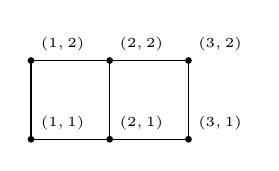
\begin{tikzpicture}
			\draw[step=1.0,black,thin] (1,1) grid (3,2);
			\foreach \x in {1,...,3}
			\foreach \y in {1,2}
			\filldraw (\x,\y) circle[radius=1pt] node[above right] {\tiny $(\x,\y)$};
		\end{tikzpicture}
	\end{center}
\end{example}

\dfn{Terna ordinata}{\index{Terna ordinata}
	Si definisce una \textbf{terna ordinata} $(a,b,c)$ come una coppia ordinata in cui la prima coordinata è una coppia ordinata $(a,b)$ e come seconda coordinata $c$:
	\begin{equation}
		\forall a,b,c \qquad (a,b,c) = \bigl((a,b),c\bigr)
	\end{equation}
}

\begin{propbox}\label{prop_terne_ordinate}
	Due terne ordinate $(a,b,c)$ e $(d,e,f)$ sono uguali se e solo se:
	\begin{equation}
		\forall a,b,c,d,e,f \qquad \bigl((a,b),c\bigr) = \bigl((d,e),f\bigr) \iff (a=d \wedge b=e \wedge c=f)
	\end{equation}
\end{propbox}

\begin{proof}
	L'enunciato si dimostra facilmente ponendo $(a,b)=m$ e $(d,e)=n$. In questo modo la dimostrazione si riduce alla dimostrazione già vista delle coppie ordinate $(m,c)$ e $(n,f)$. 
\end{proof}
\newpage
\section{Esercizi svolti}
\begin{exsbox}
	Verificare $3 \in \{2n^{2}+1 \; | \; n \in \mathbb{Z}\}$.
\end{exsbox}
\paragraph{Svolgimento.} Poniamo $A=\{2n^{2}+1 / n \in \mathbb{Z}\}$. Per essere verificata l'appartenenza deve valere la seguente equivalenza logica
\begin{displaymath}
	3 \in A \iff \exists n \in \mathbb{Z}(3=2n^{2}+1)
\end{displaymath}
e procediamo sviluppando algebricamente tale relazione fino ad ottenere una relazione più semplice da valutare:
\begin{align*}
	3 \in A &\iff \exists n \in \mathbb{Z}(3=2n^{2}+1)\\
	&\iff \exists n \in \mathbb{Z}(2=2n^{2}) & \text{\textcolor{gray}{Spostando 1 a sinistra}}\\
	&\iff \exists n \in \mathbb{Z}(n^{2}=1) & \text{\textcolor{gray}{Semplificando}}
\end{align*}
L'ultima equivalenza è chiaramente vera in quanto, per $n=\pm 1 \in \mathbb{Z}$ si ha $n^{2}=1$. Quindi $3 \in A$. \hfill \blacksquare
\begin{exsbox}
	Sia $A= \{\{a,b\}/a,b \in \mathbb{Z}\}$ un insieme. Verificare $\{1\} \in A$ e $\{1,2,3\} \in A$.
\end{exsbox}
\paragraph{Svolgimento.} Chiaramente:
\begin{align*}
	\{1\} \in A \iff \exists a,b \in \mathbb{Z}(\{a,b\} = \{1\})
\end{align*}
che risulta vera per $a=b=1$. Infatti $\{1,1\}=\{1\} \in A$. Al contrario, non esistono due numeri interi relativi tali che $\{a,b\}=\{1,2,3\}$ in quanto tale insieme contiene 3 elementi mentre $\{a,b\}$ ne può contenere al massimo due (quando $a \neq b$). Quindi $\{1,2,3\} \notin A$. \hfill \blacksquare
\begin{exsbox}
	Sia $f=\{\{a,b\},\{b,d\}\}$. Si calcolino $\bigcap f$ e $\bigcup f$.
\end{exsbox}
\paragraph{Svolgimento.} L'intersezione unaria di $f$ è definita come l'insieme degli elementi appartenenti a ciascun elemento di $f$, ovvero:
\begin{displaymath}
	\bigcap f = \{x / \forall y \in f (x \in y)\} = \{a,b\} \cap \{b,d\}= \{b\}
\end{displaymath}
\marker{yellow!50}{yellow!20!black}{Non dimenticare che $b \neq \{b\}$, nel primo caso ci si sta riferendo all'entità $b$ mentre nel secondo al singleton dell'entità $b$. \emph{Sarebbe stato un errore} scrivere quindi $\bigcap f = b$.}
Nel caso dell'unione unaria abbiamo che:
\begin{displaymath}
	\bigcup f = \{x / \exists y \in f (x \in f)\} = \{a,b\} \cup \{b,d\} = \{a,b,d\}
\end{displaymath}
\hfill \blacksquare
\begin{exsbox}
	Sia $A$ l'insieme dei numeri pari e $B$ quello dei numeri naturali moltiplicati per 2; dire in quale relazione stanno i due insiemi.
\end{exsbox}
\paragraph*{Svolgimento.} Per definizione di numero pari esprimiamo l'insieme $A$ come: $$\{p \in \mathbb{Z} / \exists k \in \mathbb{Z}(p = 2k)\}$$ mentre $$B= \{m \in \mathbb{N} / \exists k \in \mathbb{N} (m = 2k) \}$$ Ovviamente vale $B \subset A$. \hfill \blacksquare
\begin{exsbox}
	Decidere se esistono e, nel caso, descrivere esplicitamente gli insiemi:
	\begin{enumerate}
		\item $\{x | \forall y(x=y) \} $
		\item $\{ x|\forall y(x \neq y) \}$
		\item $ \{ x| \exists y (x=y)\}$
		\item $\{x|\exists y(x \neq y)\}$
		\item $ \{ x| \forall y (y \subseteq x) \}$
		\item $\{x|x=\{0,1,2\} \}$
		\item $\{y|y=\{0,1,2\} \}$
		\item $\{ x | x= \{0,1,2,x \} \}$
	\end{enumerate}
\end{exsbox}
\paragraph*{Svolgimento.} Si ha:
\begin{enumerate}
	\item  $\{x | \forall y(x=y) \} = \varnothing$. Non esiste infatti un insieme $x$ che sia uguale a tutti gli insiemi $y$. Quindi non esiste nessun elemento in questo insieme. Quindi l'insieme è l'insieme vuoto.
	\item $\{x|\forall y(x \neq y)\}= \varnothing$. Infatti non è vero che per ogni $x$, comunque si prenda un insieme $y$ allora $x \neq y$ perché appunto si potrebbe scegliere $x$ stesso al posto di $y$ ottenendo la proposizione ``$\forall x(x \neq x)$'' e poiché ogni oggetto è uguale a stesso allora si può dire che non esistono oggetti che appartengono alla totalità descritta dalla formula e per questo motivo l'insieme descrive l'insieme vuoto.
	\item Va notato che la proprietà di questo insieme è la negazione dell'insieme precedente. Per questo motivo possiamo dire che la proprietà è vera in quanto è vero che esiste almeno un insieme tale per cui sia uguale ad $x$ (ovvero $x$ stesso). Essendo vera questa formula allora sarebbe vero che per ogni insieme $x$ questo appartiene all'insieme $A=\{x|\exists y(x=y)\}$ ma non esistendo l'insieme di tutti gli insiemi allora l'insieme in questione non esiste.
	\item Analogamente come nell'esercizio precedente.
	\item L'insieme $\{x|\forall y(y \subseteq x)\}$ rappresenta l'insieme vuoto. Infatti non esiste un insieme tale per cui, comunque si scelga un insieme $y$, esso sia parte di $x$. Per fugare ogni dubbio, per rendere evidente che questa proposizione è false basta trovare un controesempio: preso l'insieme $x$ è immediato osservare che il singleton $\{x\}$ non è contenuto in $x$:$\forall x \bigl(\{x\} \nsubseteq x \bigr)$.
	\item L'insieme $\{x|x=\{0,1,2\}\}$ esiste ed ha un solo elemento. Infatti, per l'assioma di estensionalità, l'insieme delle $x$ tali che $x=\{0,1,2\}$ è il singleton di siffatto insieme $x$. Quindi:
	\begin{displaymath}
		\{x|x=\{0,1,2\}\} = \bigl\{ \{0,1,2\}  \bigr\}
	\end{displaymath}
	\item Uguale all'insieme precedente.
	\item $A=\{x|x=\{0,1,2,x\}\}=\varnothing$. Infatti si deve avere $\forall x(x \in A \iff \varphi)$, dove $\varphi$ rappresenta il predicato ``$x=\{0,1,2,x\}$''. Questa condizione è falsa per ogni $x$ in quanto nessun insieme appartiene a sé stesso e quindi l'insieme $A$ è vuoto. \hfill \blacksquare
\end{enumerate}
\begin{exsbox}
	Dire quali delle seguenti relazioni sono vere e quali false:
	\begin{enumerate}
		\item $\{1,3,5,10\} = \{3,1,10,5\}$;
		\item $\{a,b,d\}=\{b,d,a\}$;
		\item $\{2,5,6\} = \{2,7,5\}$;
		\item $\{a\} = a$;
		\item $a \in \{a\}$;
	\end{enumerate}
\end{exsbox}
\paragraph{Svolgimento.} Si ha:
\begin{enumerate}
	\item Vero
	\item Vero
	\item Falso
	\item Falso
	\item Vero \hfill \blacksquare
\end{enumerate}
\begin{exsbox}
	Sia $x=\{\{\{\{\varnothing\}\}\}\}$. Quanti elementi ha $x$? Quante parti ha $x$?
\end{exsbox}
\paragraph{Svolgimento.} L'insieme $x$ ha un solo elemento, di conseguenza l'insieme delle parti avrà solo le parti banali. \hfill \blacksquare
\begin{exsbox}
	Vero o falso?
	\begin{enumerate}
		\item $\varnothing \in \varnothing$
		\item $\varnothing \subseteq \varnothing$
		\item $\varnothing \subset \varnothing$
		\item $\varnothing \in \mathcal{P}(\varnothing)$
		\item $\varnothing \subseteq \mathcal{P}(\varnothing)$
		\item $\varnothing = \{\varnothing\}$
		\item $\varnothing \subseteq \{\varnothing\}$
		\item $\varnothing \in \{\varnothing\}$
		\item $\{1,1,2,2,2,3,3\}$ è una parte di $\{2,1,3\}$
		\item $\{1,1,2,2,2,3,3\}$ è una parte di $\{4,2,1,3\}$
	\end{enumerate}
\end{exsbox}
\paragraph{Svolgimento.} Si ha:
\begin{enumerate}
	\item Falso
	\item Vero
	\item Falso
	\item Vero
	\item Vero
	\item Falso
	\item Vero
	\item Vero
	\item Vero
	\item Vero. \hfill \blacksquare
\end{enumerate}
\begin{exsbox}
	Elencare gli elementi di $\mathcal{P}(\{0,1,2\})$.
\end{exsbox}
\paragraph{Svolgimento.}
Si ha $\mathcal{P}(\{0,1,2\})=\bigl\{ \varnothing, \{0,1,2\},\{ 0\},\{1\},\{2\},\{1,2\},\{0,1\},\{0,2\}   \bigr\} $.
\hfill \blacksquare

\begin{exsbox}
	Illustrare con i grafici di Eulero Venn la proprietà transitiva dell'inclusione tra i seguenti insiemi:
	\begin{displaymath}
		\begin{array}{lll}
			A = \{2,3,5\} & B= \{2,3,8,5\} & C = \{3,2,8,5,10,12\}
		\end{array}
	\end{displaymath}
\end{exsbox}
\paragraph{Svolgimento.} Si ha:
\begin{center}
	\includegraphics[scale=.45]{res/Venn_Esercizio1}
\end{center}
\hfill \blacksquare
\begin{exsbox}
	Determinare rispetto a $\mathbb{Z}$ gli insiemi complementari dei seguenti insiemi:
	\begin{enumerate}
		\item $\{x / x \in \mathbb{Z} \land x <3\}$
		\item $\{x / x \in \mathbb{Z} \land 2 \leq x \leq 5 \}$
		\item $\{x / x \in \mathbb{Z} \land 1 < x < 5 \}$
		\item $\{x / x \in \mathbb{Z} \land 1 \leq x \leq 2 \}$
		\item $\{x / x \in \mathbb{Z} \land x \geq 1 \}$
		\item $\{x / x \in \mathbb{Z} \land x \leq 0 \}$
	\end{enumerate}
\end{exsbox}
\paragraph{Svolgimento.} Definiamo complemento di una parte $X$ di un insieme non vuoto $S$ la differenza $S \setminus X$. Abbiamo allora:
\begin{enumerate}
	\item $\mathbb{Z} \setminus \{x / x \in \mathbb{Z} \land x <3\} = \{x / x \in \mathbb{Z} \land x > 3\}$;
	\item $\mathbb{Z} \setminus \{x / x \in \mathbb{Z} \land 2 \leq x \leq 5 \} = \{x / x \in \mathbb{Z} \land x < 2 \land x > 5\}$;
	\item $\mathbb{Z} \setminus \{x / x \in \mathbb{Z} \land 1 < x < 5 \} = \{x / x \in \mathbb{Z} \land x \leq 1 \land x \geq 5\}$;
	\item $\mathbb{Z} \setminus \{x / x \in \mathbb{Z} \land 1 \leq x \leq 2 \} = \{x /  x \in \mathbb{Z} \land x < 1 \land x > 2\}$;
	\item $\mathbb{Z} \setminus \{x / x \in \mathbb{Z} \land x \geq 1 \} = \{x / x \in \mathbb{Z} \land x < 1 \}$;
	\item $\mathbb{Z} \setminus \{x / x \in \mathbb{Z} \land x \leq 0 \} = \{x / x \in \mathbb{Z} \land x > 0 \}$. \hfill \blacksquare
\end{enumerate}
\begin{exsbox}
	L'insieme $\mathbb{Z}$ appartiene a $\mathcal{P}(\mathbb{Z})$?
\end{exsbox}
\paragraph{Svolgimento.} Sì. In ogni insieme $S \neq \emptyset$ si ha che $\emptyset$ ed $S$ sono parti banali e appartengono a $\mathcal{P}(S)$. \hfill \blacksquare
\begin{exsbox}
	Descrivere esplicitamente gli insiemi:
	\begin{enumerate}
		\item $\{x | \forall y (x \cap y = \varnothing)\}$
		\item $\{x | \exists y (x \cup y = \varnothing)\}$
		\item $\{x | \forall y (x \cup y = \varnothing)\}$
	\end{enumerate}
\end{exsbox}
\paragraph{Svolgimento.} Si ha:
\begin{enumerate}
	\item $\{x | \forall y (x \cap y = \varnothing)\}=\{ \varnothing \}$. Infatti l'insieme rappresenta l'insieme degli insiemi che non hanno alcun elemento in comune con tutti gli insiemi. L'unico insieme a soddisfare questa proprietà è l'insieme vuoto.
	\item $\{x | \exists y (x \cup y = \varnothing)\} = \{ \varnothing\}$. Infatti l'insieme rappresenta l'insieme di tutti gli insiemi $x$ per i quali esiste almeno un insieme $y$ tale che l'unione con $x$ sia il vuoto. L'unico insieme a soddisfare tale proprietà è l'insieme vuoto in quanto $\varnothing \cup \varnothing = \varnothing$.
	\item $\{x | \forall y (x \cup y = \varnothing)\}= \varnothing$. Infatti non esiste un insieme per cui la sua unione con qualsiasi insieme sia uguale all'insieme vuoto. \hfill \blacksquare
\end{enumerate}
\begin{exsbox}
	Per quali coppie di insiemi $a$, $b$, si ha $a \setminus b = b \setminus a$?
\end{exsbox}
\paragraph{Svolgimento.} L'unico caso in cui $a \setminus b$ può essere uguale a $b \setminus a$ è quando $a=b$. Infatti si ha $a \setminus b = \varnothing = b \setminus a$. \hfill \blacksquare
\begin{exsbox}
	Rappresentare, in diagrammi di Venn generici, i termini insiemistici $a \setminus ( b \setminus c)$ e $(a \setminus b) \setminus c$. Decidere se è vera o falsa la proposizione: $(\forall a,b,c)(a \setminus(b \setminus c) = (a \setminus b) \setminus c)$. Ripetere l'esercizio per $a \cap (b \setminus c)$ e $(a \cap b)\setminus c$.
\end{exsbox}
\paragraph{Svolgimento.}
L'insieme $a\setminus(b\setminus c)$ è rappresentato dal diagramma di Venn \ref{fig:venn228} mentre l'insieme $(a\setminus b)\setminus c$ dal diagramma \ref{fig:venn2282}.
\begin{center}
	\begin{minipage}{.45\textwidth}
		\centering
		\includegraphics[scale=0.6]{res/path33251.png}
		\captionof{figure}{}\label{fig:venn228}
	\end{minipage}
	\hfil
	\begin{minipage}{.45\textwidth}
		\centering
		\includegraphics[scale=0.6]{res/path2879.png}
		\captionof{figure}{}\label{fig:venn2282}
	\end{minipage}
\end{center}
Osservando i due diagrammi possiamo concludere che la differenza simmetrica tra tre insiemi non gode della proprietà associativa. Non è vero dunque che:
$\forall \ a,b,c \Bigl(a \setminus (b\setminus c) = (a \setminus b) \setminus c \Bigr)$. Analogamente, i diagrammi di Eulero Venn \ref{fig:venn2283} e \ref{fig:venn2284} rappresentano gli insiemi $a\cap(b \setminus c)$ e $(a \cap b) \setminus c$.
\begin{center}
	\begin{minipage}{.45\textwidth}
		\centering
		\includegraphics[scale=0.5]{res/Venn2882.png}
		\captionof{figure}{}\label{fig:venn2283}
	\end{minipage}
	\hfil
	\begin{minipage}{.45\textwidth}
		\centering
		\includegraphics[scale=0.5]{res/Venn2882_2.png}
		\captionof{figure}{}\label{fig:venn2284}
	\end{minipage}
\end{center}
Dai due diagrammi ci si può convincere del fatto che: $\forall \ a,b,c \Bigl(a\cap(b \setminus c) = (a \cap b) \setminus c \Bigr)$. \hfill \blacksquare
\begin{exsbox}
	Rappresentare in diagramma di Eulero Venn $(a \triangle b) \triangle c$.
\end{exsbox}
\paragraph*{Svolgimento.}
Si ha che $(a \setminus b)\setminus c$ è uguale al seguente diagramma di Eulero Venn:
\begin{center}
	\includegraphics[scale=0.6]{res/diff3sim.png}
\end{center}

Infatti, posto $\alpha= x \in A$, $\beta=x \in B$ e $\gamma=x\in C$ si ha:
\begin{displaymath}
	x \in	(a \triangle b)\triangle c \iff \bigl( \alpha \xor \beta \bigr) \xor \gamma
\end{displaymath}
Che, per la tautologia \ref{eq:xor2} è equivalente all'implicazione:
\begin{displaymath}
	(\alpha \iff \beta) \iff \gamma
\end{displaymath}
che è vera quando vale una e una sola delle tre proprietà (come evidenziato dalle zone in verde alle estremità del diagramma) oppure valgono contemporaneamente (la parte centrale del diagramma).  \hfill \blacksquare

\begin{exsbox}
	Dimostrare che, per ogni $a$, $b$ sono equivalenti tra loro:
	\begin{enumerate}
		\item $a \subseteq b$
		\item $a \cap b = a$
		\item $a \cup b = b$
	\end{enumerate}
\end{exsbox}
\paragraph{Svolgimento.} ($1 \implies 2$) Dire che per ogni insieme $a$ e $b$ si ha $a \subseteq b$ significa affermare:
\begin{displaymath}
	\forall x (x \in a \implies x \in B)
\end{displaymath}
Poiché l'intersezione tra i due insiemi è l'insieme che contiene gli elementi in comune tra i due è evidente che l'insieme formato sia $a$.

($1 \implies 3$) Analogamente, se $a$ è un sottoinsieme di $b$ e l'unione è l'insieme formato da tutti gli elementi che si trovano o in $a$ o in $b$ allora l'unione tra i due insiemi è $b$ stesso.

($3 \implies 1$) Se $a \cup b = \{x | x \in a \lor x \in b\} = b$ può significare solo due cose. O che $a$ è l'insieme vuoto o che $a$ è un sottoinsieme di $b$. In entrambi i casi si ha $a \subseteq b$. \hfill \blacksquare

\begin{exsbox}
	Calcolare, per un arbitrario insieme $a$:
	\begin{enumerate}
		\item $a \triangle a$
		\item $a \triangle \emptyset $
	\end{enumerate}
\end{exsbox}
\paragraph{Svolgimento.} Per definizione di differenza simmetrica si ha:
\begin{align*}
	a \triangle a &= \{ x \; | \; x \in \bigl(( a \cup a) \setminus (a \cap a)\bigr) \}  \\
	&= \{x \; | \; x \in (a \setminus a) \} \\
	&= \varnothing
\end{align*}
mentre nel caso della seconda formula:
\begin{align*}
	a \triangle \varnothing &= \{ x \; | \; x \in \bigl(( a \cup \varnothing ) \setminus (a \cap \varnothing)\bigr) \} \\
	&= \{x \; | \; x \in (a \setminus \varnothing ) \} \\
	&= a
\end{align*}
\hfill \blacksquare

\begin{exsbox}
	Rappresentare, in un diagramma di Venn generico, il termine insiemistico $A \cap ( B \triangle C)$.
\end{exsbox}
\paragraph{Svolgimento. }Si procede calcolando innanzitutto $B \triangle C$ (la zona evidenziata di grigio) e poi si calcola l'intersezione con l'insieme $A$. Si ottiene così il diagramma di Venn mostrato in figura:
\begin{center}
	\includegraphics[scale=.6]{res/Venn_Esercizio2.png}
\end{center}
\hfill \blacksquare
\begin{exsbox}
	Rappresentare su un diagramma di Venn di tipo generale l'espressione insiemistica:
	$(A \setminus B) \triangle (B \cup C)$.
\end{exsbox}
\paragraph{Svolgimento.} Si ha:
\begin{align*}
	(A \setminus B) \triangle (B \cup C) &= \bigl((A \setminus B)  \cup (B \cup C)\bigr) \setminus \bigl((A \setminus B) \cap (B \cup C)\bigr) \\
\end{align*}
\begin{center}
	\includegraphics[scale=.6]{res/Venn_Esercizio3.png}
\end{center}
\hfill \blacksquare
\begin{exsbox}
	Rappresentare, in un diagramma di Venn generico, i termini insiemistici $A \cup (B \cap C)$ e $A \cap (B \cup C)$. Decidere se vale una delle formule:
	\begin{eqnarray}
		\forall A,B,C (A \cup (B \cap C) \subseteq A \cap (B \cup C))  \\
		\forall A,B,C (A \cup (B \cap C) \supseteq A \cap (B \cup C))
	\end{eqnarray}
\end{exsbox}
\paragraph{Svolgimento.}
Si ha $A \cup (B \cap C)$ rappresentato in figura \ref{fig:venn4} mentre $A \cap (B \cup C)$ è mostrato in Figura \ref{fig:venn5}.
\begin{center}
	\begin{minipage}{.45\textwidth}
		\centering
		\includegraphics[scale=.6]{res/Venn_Esercizio4.png}
		\captionof{figure}{$A \cup (B \cap C)$}\label{fig:venn4}
	\end{minipage}
	\hfil
	\begin{minipage}{.45\textwidth}
		\centering
		\includegraphics[scale=.6]{res/Venn_Esercizio5.png}
		\captionof{figure}{$A \cap (B \cup C)$}\label{fig:venn5}
	\end{minipage}
\end{center}
Osservando i diagrammi di Venn possiamo dire con certezza che $\forall A,B,C (A \cup (B \cap C) \supseteq A \cap (B \cup C))$. \hfill \blacksquare
\begin{exsbox}
	Rappresentare con un diagramma di Eulero Venn l'insieme: $\Bigl( \bigl(   (a \triangle b) \triangle c \bigr) \triangle d \Bigr)$.
\end{exsbox}
\paragraph{Svolgimento.} Affermare che un qualsiasi $x$ appartiene all'insieme $\Bigl( \bigl( (a \triangle b) \triangle c \bigr) \triangle d   \Bigr)$ è equivalente alla seguente catena di implicazioni:
\begin{align*}
	\forall x \biggl( x \in \Bigl( \bigl( (a \triangle b) \triangle c \bigr) \triangle d   \Bigr) \biggr) &\iff \forall x \Bigl( x \in \bigl( (a \triangle b) \triangle c \bigr) \xor (x \in d) \Bigr) \\
	&\iff \forall x \Bigl( \bigl( x \in (a \triangle b) \xor x \in c  \bigr) \xor (x \in d)        \Bigr) \\
	&\iff \forall x \Bigl( (x \in a) \xor (x \in b) \xor (x \in c) \xor (x \in d)   \Bigr)
\end{align*}
che è vera quando è vera singolarmente una delle condizioni di appartenenza oppure quando vale per tre di esse. Quindi l'insieme così ottenuto è quello evidenziato dalle strisce nel diagramma di Eulero Venn mostrato nella Figura \ref{fig:venn215}.
\begin{center}
	\includegraphics[scale=0.7]{res/path9768.png}
	\captionof{figure}{}\label{fig:venn215}
\end{center}
\begin{exsbox}
	Rappresentare, in diagrammi di Venn generici, i termini insiemistici $a \cap (b \triangle c)$ e $a \cup (b \triangle c)$, confrontandoli tra loro e con $(a \cap b) \triangle (a \cap c)$ e $(a \cup b) \triangle (a \cup c)$.
\end{exsbox}
\paragraph{Svolgimento.} Si ha:
\begin{center}
	\begin{minipage}{.45\textwidth}
		\centering
		\includegraphics[scale=.5]{res/Venn_Esercizio6.png}
		\captionof{figure}{$a \cap (b \triangle c)$}
	\end{minipage}
	\begin{minipage}{.45\textwidth}
		\centering
		\includegraphics[scale=.5]{res/Venn_Esercizio7.png}
		\captionof{figure}{$a \cup (b \triangle c)$}
	\end{minipage} \\
	\begin{minipage}{.45\textwidth}
		\centering
		\includegraphics[scale=.5]{res/Venn_Esercizio8.png}
		\captionof{figure}{$(a \cap b) \triangle (a \cap c)$}
	\end{minipage}
	\begin{minipage}{.45\textwidth}
		\centering
		\includegraphics[scale=.5]{res/Venn_Esercizio9.png}
		\captionof{figure}{$(a \cup b) \triangle (a \cup c)$}
	\end{minipage}
\end{center}
Osservando i vari diagrammi di Venn possiamo dire con certezza che vale:
\begin{displaymath}
	\begin{array}{l}
		a \cap (b \triangle c) = (a \cap b) \triangle (a \cap c)  \\
		a \cap (b \triangle c) \subset a \cup (b \triangle c) \\
		(a \cup b) \triangle (a \cup c) \subset  a \cup (b \triangle c)
	\end{array}
\end{displaymath}
\hfill \blacksquare
\begin{exsbox}
	Siano $a$ e $b$ due insiemi. Supposto $a \subseteq b$, descrivere $a \triangle b$.
\end{exsbox}
\paragraph{Svolgimento.} Per definizione
\begin{equation}\label{eq:diff_simm_parti}
	a \triangle b = (a \cup b) \setminus (a \cap b)
\end{equation}
Ma, essendo $a \subseteq b$, valgono le seguenti relazioni:
\begin{eqnarray}
	a \cup b = b \\
	a \cap b = a
\end{eqnarray}
Quindi, sostituendo tali relazioni in \ref{eq:diff_simm_parti} si ottiene:
\begin{align*}
	a \triangle b &= (a \cup b) \setminus (a \cap b) \\
	&= b \setminus a
\end{align*}
Ovvero il complemento di $a$ in $b$ come mostrato nel seguente diagramma di Venn:
\begin{center}
	\includegraphics[scale=.8]{res/Venn_Esercizio10}
\end{center}
\hfill \blacksquare
\begin{exsbox}
	Siano $A=\{n \in \mathbb{N} \; | \; 3 \leq n \leq 10\}$, $B$ l'insieme dei numeri naturali pari, $C=\{1,2,8,13,1234\}$. Descrivere, elencandone gli elementi:
	\begin{enumerate}
		\item $A\setminus B$
		\item $A \triangle C$
		\item $B \cap C$
		\item $B \triangle (B \setminus C)$.
	\end{enumerate}
\end{exsbox}
\paragraph{Svolgimento.} Abbiamo:
\begin{displaymath}
	\begin{array}{l}
		A \setminus B = \{3,5,7,9\}\\
		A \triangle C = \{1,2,4,5,6,7,9,10,13,1234\}\\
		B \cap C = \{2,8,1234\}\\
		B \triangle (B \setminus C) = \{2,8,1234\}
	\end{array}
\end{displaymath}
\marker{yellow!50}{yellow!20!black}{Sfrutta la proprietà della differenza simmetrica tra un insieme ed una sua parte dimostrata nell'esercizio precedente.}
\hfill \blacksquare
\begin{exsbox}
	Calcolare:
	\begin{enumerate}
		\item $ \bigcup \varnothing$
		\item $ \bigcup \{ \varnothing \} $
		\item $ \bigcup \{ a \}$
		\item $ \bigcap \{ a \} $
	\end{enumerate}
\end{exsbox}
\paragraph{Svolgimento.} Si ha:
\begin{align*}
	\bigcup  \varnothing &= \varnothing \\
	\bigcup  \{ \varnothing \} &= \{ x \; | \; x \in \varnothing \} = \varnothing  \\
	\bigcup  \{a \} &= \{ x \; | \; x \in \{ a \} \} = a \\
	\bigcap  \{a \} &= a
\end{align*}
\hfill \blacksquare
\begin{exsbox}
	Calcolare $\bigcap A$ e $\bigcup A$ in ciascuno dei seguenti casi:
	\begin{enumerate}
		\item A è l'insieme delle parti infinite di $\mathbb{N}$
		\item $A=\{X \subseteq \mathbb{N} \;|\; 13 \notin X \}$
		\item $A=\{X \subseteq \mathbb{N} \;|\; 13 \in X \}$
		\item $A=\{\{124,n\} \; | \; n \in \mathbb{N}\}$
		\item $A=\{[n-1,n+1] \; | \; n \in \mathbb{N}\}$ dove $[a,b]=\{x \in \mathbb{R} \; | \; a \leq x \leq b \}$
	\end{enumerate}
\end{exsbox}
\paragraph{Svolgimento.} Si ha:
\begin{enumerate}
	\item $\bigcup A = \mathbb{N}$, $\bigcap A = \varnothing$. 	Se supponiamo infatti che esista un elemento $x$ appartenente a tutte le parti infinite di $\mathbb{N}$, cioè $\bigcap A = \{x\}$. Allora $x \in \mathbb{N}$ e vale $\forall x( x \notin \mathbb{N}\setminus\{x\})$, dove $\mathbb{N}\setminus\{x\}$ è una parte infinita di $\mathbb{N}$ e il che è assurdo.
	\item $\bigcup A = \mathbb{N}\setminus \{13\}$,	$\bigcap A = \varnothing$
	\item 	$\bigcup A = \mathbb{N}$, $\bigcap A = \{13\}$
	\item 	$\bigcup A = \mathbb{N}$, $\bigcap A = \{124\}$
	\item $\bigcup A = \{x \in \mathbb{R} \; | \; x \geq -1 \} $, $\bigcap A = \varnothing$
\end{enumerate}
\hfill \blacksquare
\begin{exsbox}
	Vero o falso?
	\begin{enumerate}
		\item $(\{0\} \times \mathbb{N}) \cap (\{1\} \times \mathbb{N}) = \{0,1\} \times \mathbb{N}$
		\item $(\mathbb{N} \times \mathbb{N}) \cup \bigl((\mathbb{Z}\setminus \mathbb{N})\times (\mathbb{Z} \setminus \mathbb{N})\bigr)= \mathbb{Z} \times \mathbb{Z}$
	\end{enumerate}
\end{exsbox}
\paragraph{Svolgimento.} 	Si ha:
\begin{enumerate}
	\item $(\{0\}\times \mathbb{N})\cap (\{1\}\times \mathbb{N}) \neq \{0,1\}\times \mathbb{N}$. Infatti $(\{0\}\times \mathbb{N})$ rappresenta l'insieme di tutte le coppie del tipo $(0,n)$ con $n \in \mathbb{N}$ mentre $(\{1\}\times \mathbb{N})$ quello delle coppie del tipo $(1,n)$ con $n \in \mathbb{N}$ quindi la loro intersezione è sicuramente vuota.
	\item $(\mathbb{N}\times \mathbb{N})\cup \bigl((\mathbb{Z} \setminus \mathbb{N}) \times (\mathbb{Z} \setminus \mathbb{N})\bigr) \neq \mathbb{Z} \times \mathbb{Z}$. Infatti:
	\begin{displaymath}
		(\mathbb{N}\times \mathbb{N})\cup \bigl((\mathbb{Z} \setminus \mathbb{N}) \times (\mathbb{Z} \setminus \mathbb{N})\bigr) =	\{(n,m)| n,m \in \mathbb{N}\} \cup \{(-n,-m) | n,m \in \mathbb{N} \}
	\end{displaymath}
	Preso un elemento di $\mathbb{Z} \times \mathbb{Z}$, ad esempio $(1,-2)$ si vede facilmente che questo non appartiene al primo insieme. \hfill \blacksquare
\end{enumerate}

\begin{exsbox}
	Verificare che:
	\begin{enumerate}
		\item $A \setminus B = A \implies A \cap B = \emptyset$
		\item $A \setminus B = \emptyset \implies A \subseteq B$
		\item $A \cap ( B \setminus C) = (A \cap B) \setminus (A \cap C)$
	\end{enumerate}
\end{exsbox}
\paragraph{Svolgimento.}
\begin{enumerate}
	\item Supponiamo che $A \cap B \neq \emptyset$. Allora, essendo non vuoto, esiste un elemento appartenente a tale intersezione, sia esso $\overline{x} \in A \cap B$. Per definizione di intersezione si ha:
	\begin{displaymath}
		\overline{x} \in A \cap B \iff x \in A \land x \in B
	\end{displaymath}
	Consideriamo adesso la differenza $A \setminus B$ definito come:
	\begin{displaymath}
		A \setminus B = \{x / x \in A \land x \notin B \}
	\end{displaymath}
	ovviamente si ha che $\overline{x} \notin A \setminus B$. Per questo e per la generalità di $\overline{x}$ possiamo affermare quindi che $A \cap B \nsubseteq A \setminus B$. Sapendo che l'intersezione tra due insiemi è sempre una parte di entrambi gli insiemi, affermare che $A \cap B \nsubseteq A \setminus B$ equivale a dire che $A \setminus B \neq A$ in quanto da tale insieme mancano sicuramente gli elementi appartenenti a $A \cap B$. Per contrapposizione si ha la tesi.
	\item Supponiamo che $A$ non sia una parte di $B$. Per definizione di sottoinsieme abbiamo che:
	\begin{align}
		A \subseteq B &\iff \forall x \in A (x \in B)
	\end{align}
	Allora, negando:
	\begin{align*}
		A \nsubseteq B &\iff \neg \bigl(\forall x (x \in A \implies x \in B)\bigr)\\
		&\iff \exists x ( x \in A \land x \notin B) & \text{\textcolor{gray}{Negando il quantificatore universale}} \\
		&\iff \exists x \in A \setminus B & \text{\textcolor{gray}{Per definizione di differenza}} \\
	\end{align*}
	Quindi $A \setminus B \neq \emptyset$. Per contrapposizione si ottiene la tesi.
	\item Dimostriamo innanzitutto che $A \cap (B \setminus C) \subseteq (A \cap B) \setminus (A \cap C)$. Sia $x \in A \cap (B \setminus C)$ allora $x$ appartiene sia ad $A$ che a $B \setminus C$, ovvero $x$ appartiene sia ad $A$ che a $B$ ma non appartiene a $C$. Pertanto $x$ appartiene a ciascuna delle differenze $A \setminus C$ che $B \setminus C$. Da $x \in A \setminus C$ possiamo osservare che sicuramente $x \notin A \cap C$ e vale quindi $x \in (A \cap B) \setminus (A \cap C)$, ovvero vale: $A \cap (B \setminus C) \subseteq (A \cap B) \setminus (A \cap C)$.
	
	Viceversa, se $x \in (A \cap B) \setminus (A \cap C)$, si ha che $x$ appartiene a $A \cap B$ e $x \notin (A \cap C)$ per cui $x$ non appartiene ad almeno uno degli insiemi $A$ e $C$. Se $x \in A \cap B$ sicuramente deve essere $x \notin C$ e allora si ha che $x \in A \land x \in B \land x \notin C$, per associatività quindi: $x \in A \cap (B \setminus C)$ e la tesi è dimostrata avendo ottenuto la doppia inclusione. \hfill \blacksquare
\end{enumerate}
\begin{exsbox}
	Si dimostri che se $B$ è un insieme e $A \subseteq B$ allora $(B \setminus A) \cap A = \emptyset $ e $(B \setminus A) \cup A = B$.
\end{exsbox}
\paragraph{Svolgimento.} Per dimostrare che un certo insieme è vuoto conviene ragionare per assurdo, cioè supporre che non sia vuoto e dedurne una contraddizione. Ad esempio, siano $A \subseteq B$ due insiemi e supponiamo per assurdo che $(B \setminus A) \cap A \neq \emptyset$. Da $(B \setminus A) \cap A \neq \emptyset$ segue che $\exists x \in (B \setminus A) \land x \in A$. Ne segue che $x \notin A$ e $x \in A$ e questa è una contraddizione. Abbiamo così dimostrato che deve essere $(B \setminus A) \cap A = \emptyset$.

Mostriamo ora che se $A \subseteq B$, allora $(B \setminus A) \cup A = B$. Dato che $B \setminus A \subseteq B$ e $A \subseteq B$, abbiamo che $(B \setminus A) \cup A  \subseteq B$. Per mostrare che $B \subseteq (B \setminus A) \cup A$ fissiamo $b \in B$. Allora si possono avere i due casi $b \in A$ oppure $b \notin A$. Se $b \in A$, allora $b \in (B \setminus A) \cup A$. Se invece $b \notin A$, si ha che $b \in B \setminus A$, e quindi $b \in (B \setminus A) \cup A$. In entrambi i casi si ha pertanto che $b \in (B \setminus A) \cup A$ e quiesto prova che $B \subseteq (B \setminus A) \cup A$. \hfill \blacksquare
\begin{exsbox}
	Siano $a$ e $b$ due insiemi. Si ha $a \times b = b \times a$ se e solo se ...?
\end{exsbox}
\paragraph{Svolgimento.} Dati due insiemi $a$ e $b$ si ha che $a \times b = b \times a $ se e solo se $a = b$. Essendo la condizione banalmente sufficiente\footnote{Si veda l'osservazione \ref{oss:condizionenecessariasufficiente}} dimostriamo che essa è necessaria, ovvero $a \times b = b \times a \implies a=b$. Prendiamo un qualsiasi elemento $x \in a$. Se $y \in b$ allora la coppia $(x,y)\in a \times b = b \times a$. Allora $x$ appartiene anche all'insieme $b$ e, per la sua generalità, possiamo dire che $a \subseteq b$. Analogamente per la seconda coordinata si ha che $y \in a$ e quindi $b \subseteq a$. Per la legge della doppia inclusione allora abbiamo $a=b$. \hfill \blacksquare
\begin{exsbox}
	Siano $A$ e $B$ due sottoinsiemi di $I$ e sia $B'$ il complementare di $B$ rispetto a $I$. Verificare che $A \setminus B = A \cap B'$.
\end{exsbox}
\paragraph*{Svolgimento.} Confrontando i due diagrammi di Venn si ha la verifica dell'asserto:
\begin{center}
	\begin{minipage}{.45\textwidth}
		\centering
		\includegraphics[scale=.6]{res/Venn_Esercizio11}
	\end{minipage}
	\hfil
	\begin{minipage}{.45\textwidth}
		\centering
		\includegraphics[scale=.6]{res/Venn_Esercizio12}
	\end{minipage}
\end{center}
Si può arrivare alla stessa conclusione osservando che un elemento $x$ appartiene all'insieme $A \setminus B$ se, e soltanto se, $x$ appartiene ad $A$ ma non appartiene a $B$. Sfruttando il fatto che $A$ è una parte di $I$ abbiamo sicuramente che $x$ è un elemento appartenente anche ad $I$, ovvero: $\forall x \in (A \setminus B) (x \in A \land x \in I \land x \notin B)$ il che è equivalente ad affermare che $x \in A \land x \in B'$ e quindi si ha che $A \setminus B \subseteq A \cap B'$. Viceversa, sia $x \in A \cap B'$. Si ha ovviamente che $x$ appartiene sia ad $A$ che al complemento di $B$, ovvero $I \setminus B$. Quindi $x \in A$, $x \in I$ e $x \notin B$. Allora $x$ appartiene ad $A$ e non appartiene a $B$, ovvero $x \in A \setminus B$ e vale $A \cap B' \subseteq A \setminus B$. Dalla doppia inclusione deriva l'asserto. \hfill \blacksquare

\begin{exsbox}
	Dimostrare che, per ogni insieme $A$, $B$:
	\begin{displaymath}
		A \times B = \varnothing \iff A = \varnothing \vee B = \varnothing
	\end{displaymath}
\end{exsbox}
\paragraph{Svolgimento}
\begin{itemize}
\item[$\impliedby$] La condizione è ovviamente sufficiente.	
\item[$\implies$] Ragionando per contrapposizione, si ottiene:
\begin{displaymath}
	\forall A,B (A = \varnothing \vee B = \varnothing)
\end{displaymath}
quindi:
\begin{displaymath}
	\exists A,B (A \neq \varnothing \wedge B \neq \varnothing)
\end{displaymath}
dunque:
\begin{displaymath}
	\exists a \in A \wedge \exists b \in B
\end{displaymath}
Fissati tali $a,b$ si ottiene:	$(a,b) \in A \times B \neq \varnothing$.\hfill \blacksquare
\end{itemize}
\begin{exsbox}
	Elencare gli elementi di $\{1,2 \} \times \{1,2,3\}$, quelli di $\{1,2,3 \} \times \{1,2\}$ e quelli di $( \{1,2\} \times \{1,2,3\} ) \cap ( \{1,2,3\} \times \{1,2\})$.
\end{exsbox}
\paragraph{Svolgimento.} Si ha:
\begin{itemize}
	\item $\{1,2 \} \times \{1,2,3\} = \{(1,1),(1,2),(1,3),(2,1),(2,2),(2,3)\}$
	\item $\{1,2,3 \} \times \{1,2\} = \{(1,1),(1,2),(2,1),(2,2),(3,1),(3,2)\}$
	\item $\{1,2\} \times \{1,2,3\} ) \cap ( \{1,2,3\} \times \{1,2\}) = \{(1,1),(1,2),(2,2)\}$. \hfill \blacksquare
\end{itemize}
\begin{exsbox}
	Vero o falso?
	\begin{enumerate}
		\item $(\{0\}\times \mathbb{N}) \cup (\{1\}\times \mathbb{N}) = \{0,1\} \times \mathbb{N}$
		\item $(\mathbb{N} \times \mathbb{N}) \cup (\mathbb{Z} \setminus \mathbb{N}) \times (\mathbb{Z}\setminus \mathbb{N}) = \mathbb{Z} \times \mathbb{Z}$.
	\end{enumerate}
\end{exsbox}
\paragraph{Svolgimento.} 
\begin{enumerate}
	\item Vero, perché $(\{0\}\times \mathbb{N}) \cup (\{1\}\times \mathbb{N})$ è l'unione  tra l'insieme di tutte le coppie di prima coordinata 0 e seconda coordinata un naturale e l'insieme di tutte le coppie di prima coordinata 1 e seconda coordinata un naturale.
	\item Vero, perché $\mathbb{Z} \times \mathbb{Z}$ può essere visto come l'unione tra l'insieme delle coppie $(a,b)$ con $a,b$ entrambi positivi e l'insieme delle coppie $(c,d)$ con $c,d$ entrambi negativi. \hfill \blacksquare
\end{enumerate}
\gbox{Tecniche di dimostrazione}{red}{
	Un \textbf{teorema} è un enunciato della forma ``Se valgono $P_{1},P_{2},\ldots,P_{n}$ allora vale anche $Q$'' che equivale alla formula logica: $P_{1} \land P_{2} \land \ldots \land P_{n} \implies Q$. Le affermazioni $P_{1},P_{2},\ldots,P_{n}$ sono dette \textbf{ipotesi} mentre $Q$ è la \textbf{tesi} del teorema. Come possiamo organizzare in modo rigoroso un ragionamento e stabilire che esso costituisce la dimostrazione di un teorema? Ci sono diverse strategie dimostrative variamente utilizzate:
	\begin{itemize}
		\item  la \textbf{dimostrazione diretta} è la strategia più semplice e naturale per stabilire un teorema del tipo descritto. La dimostrazione diretta assume di trovarsi in un qualunque contesto in cui siano verificate le ipotesi e sulla base di semplici e rigorosi ragionamenti stabilisce che in tale contesto anche la tesi è verificata.
		\item la \textbf{dimostrazione per assurdo} consiste in una dimostrazione in cui si assume che la tesi sia falsa e da questa assunzione si deriva (utilizzando anche le ipotesi) una contraddizione, ovvero una proposizione della forma $p \land (\neg p)$ che asserisce che una qualche affermazione $p$ è contemporaneamente vera e falsa. Questo prova che $Q$ non può essere che vera in quanto il suo essere falso porterebbe a conclusioni assurde.
		In altre parole: si dimostra che se le premesse sono vere non è possibile che la tesi sia falsa.
		\item la \textbf{dimostrazione per contrapposizione} viene usata per dimostrare un teorema del tipo $p \implies q$ attraverso la dimostrazione (in modo diretto) del teorema: $\neg q \implies \neg p$. Infatti, supposto di aver stabilito la correttezza del teorema ``non $Q$ allora non $P$'' e di essere in un contesto in cui vale l'ipotesi $P$, allora, in tale contesto, anche $Q$ deve essere vera, perché se fosse falsa (ovvero se valesse non $Q$) allora si avrebbe che sia $P$ che non $P$ sarebbero vere, contraddizione!
	\end{itemize}
}
%  % Chapter 3: Funzioni
  \input{chapters/chapter_3.tex}
%  % Chapter 4: Combinatoria
  \input{chapters/chapter_4.tex}
%  % Chapter 5: Strutture albegriche
  \input{chapters/chapter_5.tex}
%  % Chapter 6: Reticoli
  \input{chapters/chapter_6.tex}
%  % Chapter 7: Aritmetica e polinomi
  \input{chapters/chapter_7.tex}
%  % Chapter 8: Teoria grafi
  \input{chapters/chapter_8.tex}
  % Chapter 9: Esercizi
  \input{chapters/chapter_9.tex}
  \printindex
\end{document}
